\documentclass[a4paper]{article}
\addtolength{\hoffset}
{-2.25cm}
\addtolength{\textwidth}
{5cm}
\addtolength{\voffset}
{-3.25cm}
\addtolength{\textheight}
{5.5cm}
\setlength{\parskip}{0pt}
\setlength{\parindent}{0in}

\usepackage[utf8]{inputenc}
\usepackage{microtype}
\usepackage[english]{babel}
\usepackage{fancyhdr}
\usepackage{advdate}
\usepackage{enumitem}
\usepackage{amsmath, amssymb}
\usepackage{graphicx}
\usepackage{caption}
\usepackage{subcaption}
\usepackage{float}
\usepackage{titlesec}
\usepackage{wasysym}
\usepackage{url}
\usepackage{hyperref}
\usepackage{tikz, verbatimbox}
\usepackage{fixltx2e}
\usepackage{centernot}
\usepackage{algorithm}
\usepackage{algpseudocode}
\usepackage{listings}
\usetikzlibrary{shapes.geometric, arrows}
\usetikzlibrary{positioning}
\usepackage[table]{xcolor}

\graphicspath{{./static/}}
\tikzset{every picture/.style={line width=0.75pt}} %set default line width to 0.75pt

\newcommand{\LComment}[1]{\State \(\triangleright\) \text{#1}}
\MakeRobust{\Call}
\usepackage{pdfpages}
\usetikzlibrary{positioning}

\begin{document}

\fancyhead[c]{}
\hrule \medskip
\begin{minipage}{0.295\textwidth}
\raggedright
Rishabh Indoria\\
21F3001823
\end{minipage}
\begin{minipage}{0.4\textwidth}
\centering
\LARGE
Software Testing
\end{minipage}
\begin{minipage}{0.295\textwidth}
\raggedleft
\today \hfill \\
\end{minipage}
\medskip \hrule
\bigskip

\section{Introduction}
\subsection{Motivation}
\begin{itemize}
    \item \textbf{Introduction to Software Testing} by Paul Ammann and Jeff Offutt, \textbf{The Art of Software Testing} by Glenford J. Myers, \textbf{Software Testing: A Craftsman's Approach} by Paul C. Jorgensen, \textbf{Agile Testing: A practical guide for Testers and Agile Teams} by Lisa Crispin and Janet Gregory.
    \item Software is ubiquitous; Such software should be of very high quality, offer good performance in terms of response time, performance and also have no errors.
    \item It is no longer feasible to shut down a malfunctioning system in order to restore safety.
    \item Errors in software can cost lives, huge financial losses, or simply a lot of irritation.
    \item Testing is the \textbf{predominantly used} technique to find and eliminate errors in software.
\end{itemize}
\subsection{Software Development Life Cycle}
\begin{itemize}
    \item \textbf{SDLC}: term used by the software industry to define a process for designing, developing, testing and maintaining a high quality software product.
    \item The goal is to use SDLC defined processes to develop a high quality software product that meets customer demands.
    \item \textbf{Planning}: Includes clearly identifying customer and/or market needs, pursuing a feasibility study and arriving at an initial set of requirements.
    \item \textbf{Requirements definition}: Includes documenting detailed requirements of various kinds: System-level, functional, software, hardware, quality requirements etc. They get approved by appropriate stakeholders.
    \item \textbf{Requirements analysis}: Includes checking and analyzing requirements to ensure that they are consistent, complete and match the feasibility study and market needs.
    \item \textbf{Design}: Identifies all the modules of the software product, details out the internals of each module, the implementation details and a skeleton of the testing details.
    \item \textbf{Architecture}: Defines the modules, their connections and other dependencies, the hardware, database and its access etc.
    \item \textbf{Development}: The design documents, especially that of low-level design, is used to implement the product. There are usually coding guidelines to be followed by the developers. Extensive unit testing and debugging are also done, usually by the developers. Tracking is done by project management team.
    \item \textbf{Testing}: Involves testing only where the product is thoroughly tested, defects are reported, fixed and re-tested, until all the functional and quality requirements are met.
    \item \textbf{Maintenance}: Done post deployment of product. Add new features as desired by the customer/market. Fix errors, if any, in the software product. Test cases from earlier phases are re-used here, based on need.
    \item \textbf{V-model}: It is a model that focuses on verification and validation. Follows the traditional SDLC life-cycle: Requirements, Design, Implementation, Testing, Maintenance.
    \item \textbf{Agile model}: Agile methodologies are adaptive and focus on fast delivery of features of a software product. All the SDLC steps are repeated in incremental iterations to deliver a set of features. Extensive customer interactions, quick delivery and rapid response to change in requirements.
    \item \textbf{Other Activities}: Project management, includes team management. Project documentation(Traceability matrix is a document that links each artifacts of development phase to those of other phases). Quality Inspection.
    \begin{figure}[H]
        \centering
        \begin{subfigure}[b]{0.45\textwidth}
            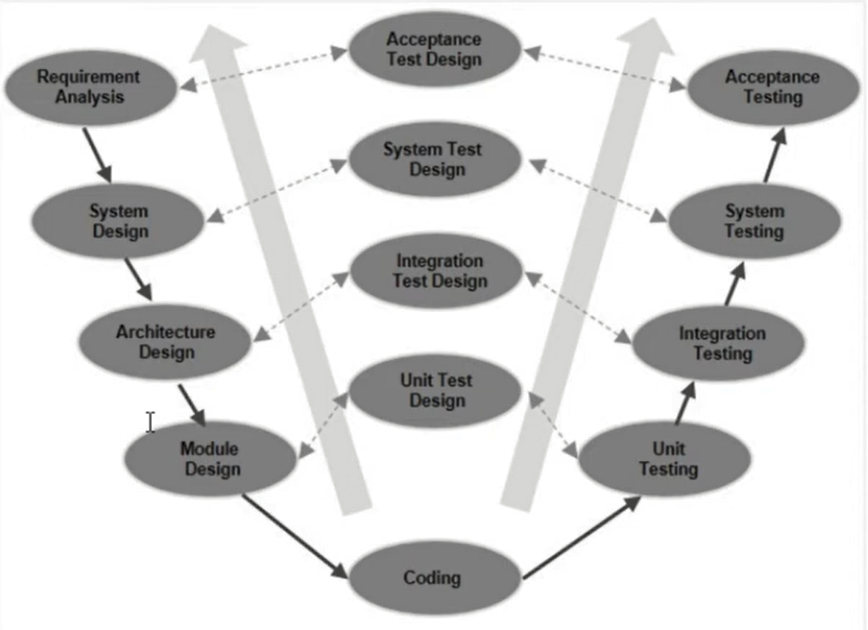
\includegraphics[width=\textwidth]{Degree/static/ST_v_model.png}
            \caption{V-Model}
            \label{fig:ST-v-model}
        \end{subfigure}
        \hfill
        \begin{subfigure}[b]{0.45\textwidth}
            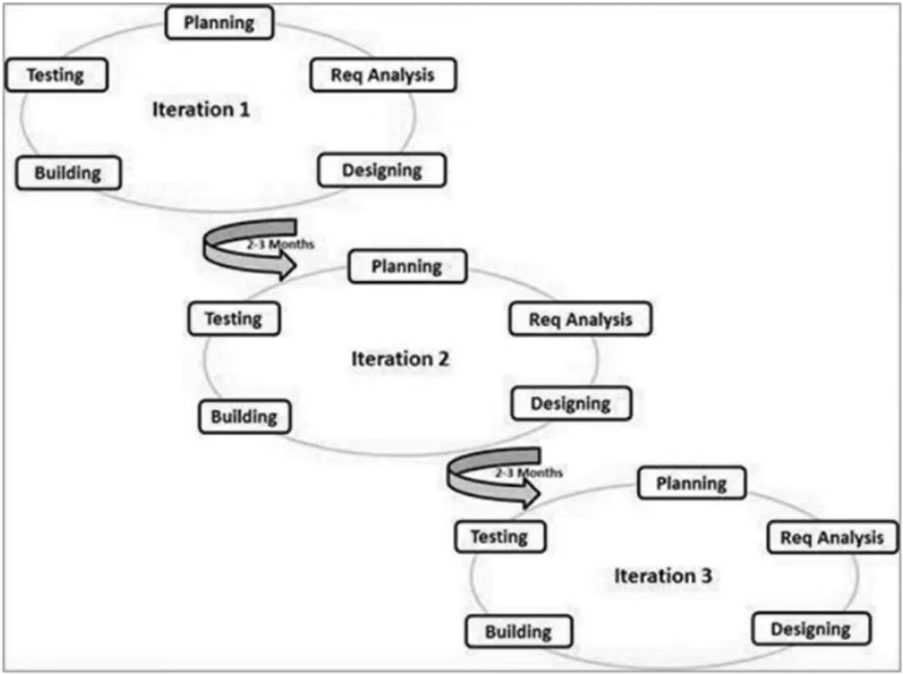
\includegraphics[width=\textwidth]{Degree/static/ST_agile_model.png}
            \caption{Agile Model}
            \label{fig:ST-agile-model}
        \end{subfigure}
        \caption{Model Visualization}
        \label{fig:ST-model-visualizations}
    \end{figure}
\end{itemize}
\subsection{Testing Terminologies}
\begin{itemize}
    \item \textbf{Validation}: The process of evaluating software at the end of software development to ensure compliance with intended usage. i.e., checking if the software meets its requirements.
    \item \textbf{Verification}: The process of determining whether the products of a given phase of the software development process fulfill the requirements established at the start of that phase.
    \item \textbf{Fault}: A static defect in the software. It could be a missing function or a wrong function in code.
    \item \textbf{Failure}: An external, incorrect behavior with respect to the requirements or other description of the expected behavior. A failure is a manifestation of a fault when software is executed.
    \item \textbf{Error}: An incorrect internal state that is the manifestation of some fault.
    \item \textbf{Test case}: A test case typically involves inputs to the software and expected outputs. A failed test case indicates an error. A test case also contains other parameters like test case ID, traceability details etc.
    \item \textbf{Unit Testing}: Done by developer during coding.
    \item \textbf{Integration Testing}: Various components are put together and tested. Components could be only software or software and hardware components.
    \item \textbf{System Testing}: Done with full system implementation and the platform on which the system will be running.
    \item \textbf{Acceptance Testing}: Done by end customer to ensure that the delivered products meet the committed requirements.
    \item \textbf{Beta Testing}: Done in a (so-called) beta version of the software by end users, after release.
    \item \textbf{Functional Testing}: Done to ensure that the software meets its specified functionality.
    \item \textbf{Stress Testing}: Done to evaluate how the system behaves under peak/unfavorable conditions.
    \item \textbf{Performance Testing}: Done to ensure the speed and response time of the system.
    \item \textbf{Usability Testing}: Done to evaluate the user interface, aesthetics.
    \item \textbf{Regression Testing}: Done after modifying/upgrading a component, to ensure that the modification is working correctly, and other components are not damaged by the modification.
    \item \textbf{Black-Box Testing}: A method of testing that examines the functionalities of a software/system without looking into its internal design or code.
    \item \textbf{White-Box Testing}: A method of testing that test the internal structure of the design or code of a software.
    \item \textbf{Test Design}: Most critical job in testing. Need to design effective test cases. Apart from specifying the inputs, this involves defining the expected outputs too. Typically, cannot be automated.
    \item \textbf{Test Automation}: Involves converting the test cases into executable scripts. Need to specify how to reach deep parts of the code using just inputs, Observability and Controllability.
    \item \textbf{Test Execution}: Involves running the test on the software and recording the results. Can be fully automated.
    \item \textbf{Test Evaluation}: Involves evaluating the results of testing, reporting identified errors. A difficult problem is to isolate faults, especially in large software and during integration testing.
    \item \textbf{Testing goals}: Organizations tend to work with one or more of the following levels\\
    \textbf{Level 0}: There is no difference between testing and debugging.\\
    \textbf{Level 1}: The purpose of testing is to show correctness.\\
    \textbf{Level 2}: The purpose of testing is to show that software doesn't work.\\
    \textbf{Level 3}: The purpose of testing is not to prove anything specific, but to reduce the risk of using the software.\\
    \textbf{Level 4}: Testing is a mental discipline that helps all IT professionals develop higher quality software.
    \item \textbf{Controllability}: Controllability is about how easy it is to provide inputs to the software module under test, in terms of reaching the module and running the test cases on the module under test.
    \item \textbf{Observability}: Observability is about how easy it is to observe the software module under test and check if the module behaves as expected.
\end{itemize}

\section{Graphs based Testing}
\subsection{Basics}
\begin{itemize}
    \item A graph is a tuple $G=(V,E)$ where $V$ is a set of \textbf{nodes/vertices}, and $E\subseteq(V\times V)$ is a set of \textbf{edges}.
    \item Graphs can be \textbf{directed} or \textbf{undirected}.
    \begin{figure}[H]
        \centering
        \begin{subfigure}[b]{0.45\textwidth}
            \centering
            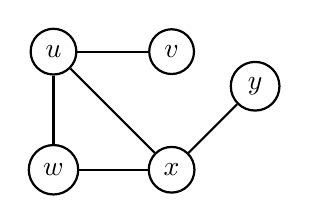
\begin{tikzpicture}[node distance={15mm}, thick, main/.style = {draw, circle}]
                \node[main] (1) {$u$};
                \node[main] (2) [right of=1] {$v$};
                \node[main] (3) [below of=1] {$w$};
                \node[main] (4) [right of=3] {$x$};
                \node[main] (5) [above right of=4] {$y$};

                \draw (1) -- (2);
                \draw (1) -- (3);
                \draw (1) -- (4);
                \draw (3) -- (4);
                \draw (4) -- (5);
            \end{tikzpicture} 
            \caption{A simple undirected graph}
        \end{subfigure}
        \hfill
        \begin{subfigure}[b]{0.45\textwidth}
            \centering
            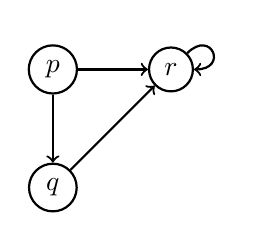
\begin{tikzpicture}[node distance={15mm}, thick, main/.style = {draw, circle}]
                \node[main] (1) {$p$};
                \node[main] (2) [right of=1] {$r$};
                \node[main] (3) [below of=1] {$q$};

                \draw[->] (1) -- (2);
                \draw[->] (1) -- (3);
                \draw[->] (3) -- (2);
                \draw[->] (2) to [out=45,in=0,looseness=5] (2);
            \end{tikzpicture} 
            \caption{A directed graph}
        \end{subfigure}
    \end{figure}
    \item Graphs can finite or infinite.
    \item The \textbf{degree} of a vertex is the number of edges that are connected to it. Edges connected to a vertex are said to be \textbf{incident} on the vertex.
    \item There are designated special vertices like \textbf{initial} and \textbf{final} vertices. These vertices indicate beginning and end of a property that the graph is modeling.
    \item Typically, there is only one initial vertex, but there could be several final vertices.
    \begin{figure}[H]
        \centering
        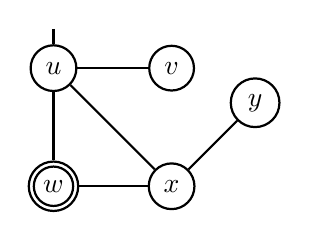
\begin{tikzpicture}[node distance={15mm}, thick, main/.style = {draw, circle}]
            \node[main] (1) {$u$};
            \node[main] (2) [right of=1] {$v$};
            \node[main] (3) [below of=1] {$w$};
            \node[main, minimum size=0.5cm] (33) [below of=1] {};
            \node[main] (4) [right of=3] {$x$};
            \node[main] (5) [above right of=4] {$y$};

            \draw (0,0.5) -- (1);
            \draw (1) -- (2);
            \draw (1) -- (3);
            \draw (1) -- (4);
            \draw (3) -- (4);
            \draw (4) -- (5);
        \end{tikzpicture}
        \caption{Graph with initial and final vertices}
    \end{figure}
    \item Most of these graphs will have \textbf{labels} associated with vertices and edges. Labels or annotations could be details about the artifact that the graphs are modelling. Tests are intended to cover the graph in some way.
    \begin{figure}[H]
        \centering
        \begin{subfigure}[b]{0.45\textwidth}
            \begin{verbatim}
                if(x<y){
                y = 0;
                x = x+1;
                }else{
                x = y+1;
                }
                z = x+1;
            \end{verbatim}
            \caption{A sample code}
        \end{subfigure}
        \hfill
        \begin{subfigure}[b]{0.45\textwidth}
            \begin{myverbbox}{\edgeONE}
                x>=y
            \end{myverbbox}
            \begin{myverbbox}{\edgeTWO}
                x<y
            \end{myverbbox}
            \begin{myverbbox}{\vertexONE}
                x = y+1
            \end{myverbbox}
            \begin{myverbbox}{\vertexTWO}
                y = 0
                x = x+1
            \end{myverbbox}
            \begin{myverbbox}{\vertexTHREE}
                z = x+1
            \end{myverbbox}
            \hspace{-2cm}
            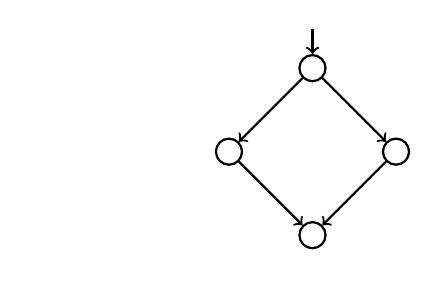
\begin{tikzpicture}[node distance={15mm}, thick, main/.style = {draw, circle}]
                \node[main] (1) {};
                \node[main] (2) [below right of=1] {};
                \node at (0.5, -1.3) {\vertexONE};
                \node[main] (3) [below left of=1] {};
                \node at (-3.5, -1.3) {\vertexTWO};
                \node[main] (4) [below left of=2] {};
                \node at (-0.5, -2.3) {\vertexTHREE};
                \node at (-0.5,-0.5) {\edgeONE};
                \node at (-2.5, -0.5) {\edgeTWO};

                \draw[->] (0,0.5) -- (1);
                \draw[->] (1) -- (2);
                \draw[->] (1) -- (3);
                \draw[->] (2) -- (4);
                \draw[->] (3) -- (4);
            \end{tikzpicture}
            \caption{A Control Flow Graph}
        \end{subfigure}
        \caption{Example of a CFG}
    \end{figure}
    \item A \textbf{path} is a sequence of vertices $v_1,v_2,...,v_n$ such that $(v_i,v_{i+1})\in E$.
    \item \textbf{Length} of a path is the number of edges that occur in it. A single vertex path has length 0.
    \item \textbf{Sub-path} of a path is a sub-sequence of vertices that occur in the path.
    \item A vertex $v$ is \textbf{reachable} from some other vertex if there is a path connecting them.
    \item An edge $e=(u,v)$ is \textbf{reachable} if there is a path that goes to vertex $u$ and then goes to vertex $v$.
    \item A \textbf{test path} is a path that starts in an initial vertex and ends in a final vertex. These represent execution of test cases.
    \item Some test paths can be executed by many test cases: \textbf{Feasible paths}.
    \item Some test paths cannot be executed by any test case: \textbf{Infeasible paths}.
    \item A test path $p$ \textbf{visits} a vertex $v$ if $v$ occurs in path $p$. A test path $p$ \textbf{visits} an edge $e$ if $e$ occurs in the path $p$.
    \item A test path $p$ \textbf{tours} a path $q$ if $q$ is a sub-path of $p$.
    \item When a test case $t$ executes a path, we call it the \textbf{test path} executed by $t$, denoted by $path(t)$.
    \item The set of test paths executed by a set of test cases $T$ is denoted by $path(T)$.
    \item \textbf{Test requirement} describes properties of test paths.
    \item \textbf{Test Criterion} are rules that define test requirements.
    \item \textbf{Satisfaction}: Given a set $TR$ of test requirements for a criterion $C$, a set of tests $T$ satisfies $C$ on a graph iff for every test requirement in $t\in TR$, there is a test path in $path(T)$ that meets the test requirement $t$.
    \item \textbf{Structural Coverage Criteria}: Defined on a graph just in terms of vertices and edges.
    \item \textbf{Data Flow Coverage Criteria}: Requires a graph to be annotated with references to variables and defines criteria requirements based on the annotations.
\end{itemize}

\subsection{Elementary Graph Algorithms}
\begin{itemize}
    \item Two standard ways of representing graphs: \textbf{adjacency matrix} or \textbf{adjacency lists}.
    \item Adjacency list representation provides a compact way to represent \textbf{sparse} graphs, i.e., graphs for which $|E|$ is much less than $|V|^2$. For each $u\in V$, $Adj[u]$ contains all vertices $v$ such that $(u,v)\in E$, i.e., it contains all edges incident with $u$. Represented in $\Theta(|V|+|E|)$ memory.
    \item Adjacency matrix representation provides a compact way to represent \textbf{dense} graphs, i.e., graphs for which $|E|$ is close to $|V|^2$. This is a $|V|\times |V|$ matrix, where $a_{ij}=1$ if there is an edge going from $i$ to $j$.
    \item \textbf{Breadth First Search}: Computes the "distance" from $s$ to each reachable vertex.
    \begin{algorithm}[H]
        \caption{Breadth First Search}\label{alg:ST-BFS}
        \begin{algorithmic}[1]
            \Statex \Call{BFS}{$G$}
            \For{each vertex $u\in G,V-\{s\}$}
                \State $u.color$ = $WHITE$, $u.d=\infty$, $u.\pi$ = NIL
            \EndFor
            \State $s.color$ = $BLUE$, $s.d=0$, $s.\pi$ = NIL
            \State $Q$ = $\phi$
            \State \Call{Enqueue}{$Q,s$}
            \While{$Q\neq \phi$}
                \State $u$ = \Call{Dequeue}{$Q$}
                \For{each $v\in G.Adj[u]$}
                    \If{$v.color$ == $WHITE$}
                        \State $v.color$ = $BLUE$
                        \State $v.d$ = $u.d$ + 1
                        \State $v.\pi$ = $u$
                        \State \Call{Enqueue}{$Q,v$}
                    \EndIf
                \EndFor
                \State $u.color$ = $BLACK$
            \EndWhile
        \end{algorithmic}
    \end{algorithm}
    \item \textbf{Depth First Search}
    \begin{algorithm}[H]
        \caption{Depth First Search}
        \begin{algorithmic}[1]
            \Statex \Call{DFS}{$G$}
            \For{each vertex $u\in G.V$}
                \State $u.color$ = $WHITE$
                \State $u.\pi$ = $NIL$
            \EndFor
            \State $time$ = 0
            \For{each vertex $u\in G.V$}
                \If{$u.color$ == $WHITE$}
                    \State \Call{DFS-Visit}{$G,u$}
                \EndIf
            \EndFor
            \Statex
            \Statex \Call{DFS-Visit}{$G,u$}
            \State $time$ = $time+1$
            \State $u.d$ = $time$
            \State $u.color$ = $GRAY$
            \For{each $v\in G.Adj[u]$}
                \If{$v.color$ == $WHITE$}
                    \State $v.\pi$ = $u$
                    \State \Call{DFS-Visit}{$G,v$}
                \EndIf
            \EndFor
            \State $u.color$ = $BLACK$
            \State $time$ = $time+1$
            \State $u.f$ = $time$
        \end{algorithmic}
    \end{algorithm}
\end{itemize}

\subsection{Structural Graph Coverage}
\begin{itemize}
    \item \textbf{Node Coverage} requires that the test cases visit each node in the graph once. Test set $T$ satisfies node coverage on graph $G$ iff for every syntactically reachable node $n\in G$, there is some path $p$ in $path(T)$ such that $p$ visits $n$.
    \item \textbf{Edge Coverage}: $TR$ contains each reachable path of length up to $1$, inclusive, in $G$. Edge coverage is slightly stronger than node coverage. Allowing length up to 1 allows edge coverage to subsume node coverage.
    \item \textbf{Edge-Pair Coverage}: $TR$ contains each reachable path of length up to 2, inclusive in $G$. Paths of length up to 2 correspond to pairs of edges.
    \item \textbf{Complete path coverage}: $TR$ contains all paths in $G$. Unfortunately, this can be an infeasible test requirement, due to loops.
    \item \textbf{Specified path coverage}: $TR$ contains a set $S$ of paths, where $S$ is specified by the user/tester.
    \item A path from $n_i$ to $n_j$ is \textbf{simple} if no node appears more than once, except possible the first and last node.
    \item A \textbf{prime path} is a simple path that does not appear as a proper sub-path of any other simple path.
    \item \textbf{Prime path coverage}: $TR$ contains each prime path in $G$. Ensures that loops are skipped as well as executed. It subsumes node and edge coverage.
    \item \textbf{Tour with side trips}: A test path $p$ tours a sub-path $q$ with side trips iff every edge $q$ is also in $p$ in the same order. the tour can include a side trip, as long as it comes back to the same node.
    \item \textbf{Tours with detours}: A test path $p$ tours a sub-path $q$ with detours iff every node in $q$ is also in $p$ in the same order. The tour can include a detour from node $n$ as long as it comes back to the prime path at a successor of $n$.
    \item \textbf{Best Effort Touring}: Satisfy as many test requirements as possible without sidetrips. Allow sidetrips to try to satisfy remaining test requirements.
    \item \textbf{Round trip path}: A prime path that starts and ends at the same node.
    \item \textbf{Simple round trip coverage}: $TR$ contains at least one round trip path for each reachable node in $G$ that begins and ends in a round trip path.
    \item \textbf{Complete round trip coverage}: $TR$ contains all round trip paths for each reachable node in $G$.
    \begin{figure}[H]
        \centering
        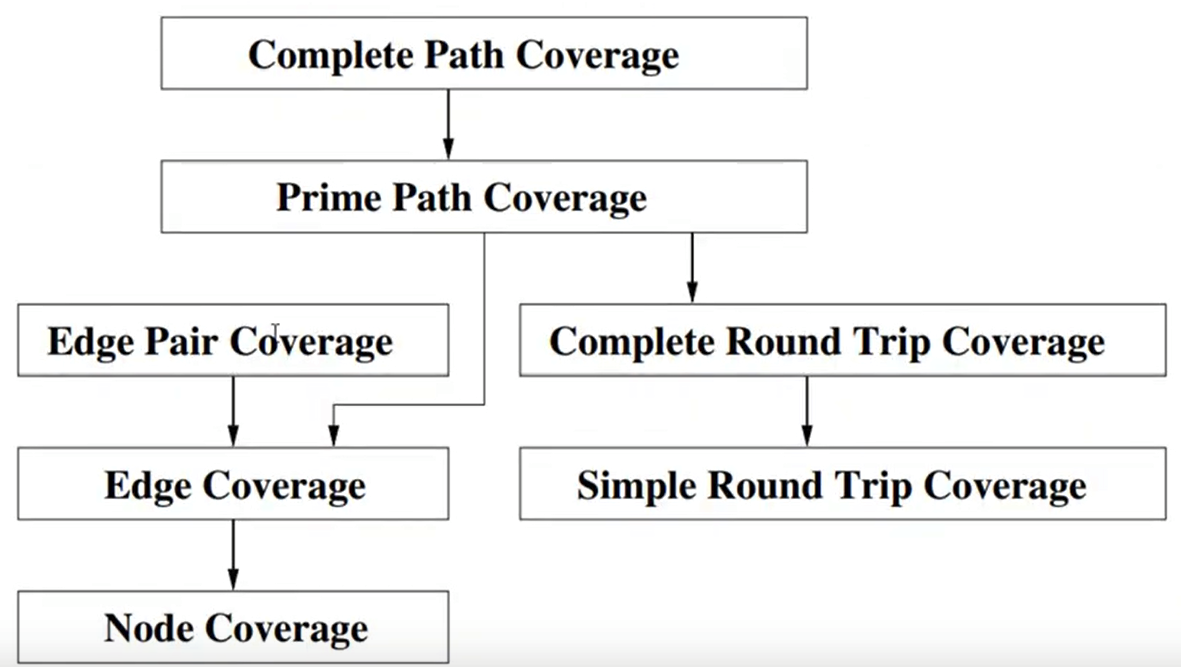
\includegraphics[width=0.5\linewidth]{Degree//static/ST_Structural_Coverage.png}
        \caption{Structure Coverage Criteria Subsumption}
        \label{fig:ST-structure-coverage}
    \end{figure}
\end{itemize}

\subsection{Algorithms: Structural Graph Coverage Criteria}
\begin{itemize}
    \item There are two entities related to coverage criteria: Test requirement, and Test case as a test path, if the test requirement is feasible.
    \item Test requirements for node and edge coverage are already given as a part of the graph modeling the software artifact. Test paths to achieve node and edge coverage can be obtained by simple modifications to BFS.
    \item $TR$ for edge-pair coverage is all paths of length two in a given graph. Need to include paths that involve self-loops too.
    \begin{algorithm}[H]
        \caption{Simple Edge-Pair Algorithm}
        \begin{algorithmic}[1]
            \For{each node $u$ in the graph}
                \For{each node $v$ in $Adj[u]$}
                    \For{each node $w$ in $Adj[v]$}
                        \State Output path $u--v--w$
                    \EndFor
                \EndFor
            \EndFor
        \end{algorithmic}
    \end{algorithm}
    \item Prime Path Algorithm
    \begin{algorithm}[H]
        \caption{Computing prime paths}
        \begin{algorithmic}[1]
            \State $Loops$ = [ ]
            \State $Terminate$ = [ ]
            \State $Stuck$ = [ ]
            \State $Q$ = $\phi$
            \For{each $v\in G$}
                \State \Call{Enqueue}{$Q,[v]$}
            \EndFor
            \While{$Q\neq \phi$}
                \State $path$ = \Call{Dequeue}{$Q$}
                \For{each $v\in G.Adj[path[-1]]$}
                    \If{$v$ is a final vertice}
                        \State $Terminate$ = $Terminate$ ++ ($path$ ++ $v$)
                    \ElsIf{$v$ in $path$ and $v$ == $path[0]$}
                        \State $Loops$ = $Loops$ ++ ($path$ ++ $v$)
                    \ElsIf{$v$ in $path$}
                        \State $Stuck$ = $Stuck$ ++ ($path$)
                    \Else
                        \State \Call{Enqueue}{$Q, path$ ++ $v$}
                    \EndIf
                \EndFor
            \EndWhile
            \LComment From these we can take the largest path as long as that path is not covered by another path.
            \State \Return $Loops$, $Terminate$, $Stuck$
        \end{algorithmic}
    \end{algorithm}
    \item To enumerate test paths for prime path coverage: Start with the longest prime paths and extend each of them to the initial and the final nodes in the graph.
\end{itemize}

\subsection{Control Flow Graphs for Code}
\begin{itemize}
    \item Modelling control flow in code as graphs. Using structural coverage criteria to test control flow in code.
    \item Typically used to test a particular function or procedure or a method.
    \item A \textbf{Control Flow Graph} models all executions of a method by describing control structures.
    \item \textbf{Nodes}: Statements or sequences of statements (basic blocks).
    \item \textbf{Basic Block}: A sequence of statements such that if the first statement is executed, all statements will be (no branches).
    \item \textbf{Edges}: Transfer of control from one statement to the next.
    \item CFGs are often annotated with extra information to model data, this includes branch predicates, Definitions and/or uses.
    \begin{figure}[H]
        \centering
        \begin{subfigure}[b]{0.45\textwidth}
            \begin{verbatim}
                x = 0;
                while(x<y){
                    y = f(x,y);
                    if(y == 0){
                        break;
                    }else if(y<0){
                        y = y*2;
                        continue;
                    }
                    x = x+1;
                }
                print(y);
            \end{verbatim}
            \caption{While loop with break and continue}
        \end{subfigure}
        \hfill
        \begin{subfigure}[b]{0.45\textwidth}
            \begin{myverbbox}{\vertexONE}
                x = 0;
            \end{myverbbox}
            \begin{myverbbox}{\edgeONE}
                x<y;
            \end{myverbbox}
            \begin{myverbbox}{\edgeTWO}
                x>=y;
            \end{myverbbox}
            \begin{myverbbox}{\vertexTWO}
                y = f(x,y);
            \end{myverbbox}
            \begin{myverbbox}{\edgeTHREE}
                y == 0;
            \end{myverbbox}
            \begin{myverbbox}{\edgeFOUR}
                y<0;
            \end{myverbbox}
            \begin{myverbbox}{\edgeFIVE}
                y>0;
            \end{myverbbox}
            \begin{myverbbox}{\vertexTHREE}
                x = x+1;
            \end{myverbbox}
            \begin{myverbbox}{\vertexFOUR}
                print(y);
            \end{myverbbox}
            \begin{myverbbox}{\vertexFIVE}
                break;
            \end{myverbbox}
            \begin{myverbbox}{\vertexSIX}
                y = y*2;
                continue;
            \end{myverbbox}
            \hspace{-2.5cm}
            \begin{tikzpicture}[node distance={15mm}, thick, main/.style = {draw, circle}]
                \node[main] (1) {1};
                \node at (-0.5, 0) {\vertexONE};
                \node[main] (2) [below of=1] {2};
                \node at (-2.2, -2.05) {\edgeONE};
                \node at (-0.3, -2.05) {\edgeTWO};
                \node[main] (3) [below right of=2] {7};
                \node at (0.8, -2.6) {\vertexFOUR};
                \node[main, minimum size=0.5cm] (33) [below right of=2] {};
                \node[main] (4) [below left of=2] {3};
                \node at (-4, -2.6) {\vertexTWO};
                \node at (-1.5, -3) {\edgeTHREE};
                \node at (-2.2, -3.6) {\edgeFOUR};
                \node at (-3.2, -3.1) {\edgeFIVE};
                \node[main] (5) [below left of=4] {5};
                \node at (-5, -3.7) {\vertexSIX};
                \node[main] (6) [below right of=4] {4};
                \node at (-0.5, -4) {\vertexFIVE};
                \node[main] (7) [below of=4] {6};
                \node at (-2, -4.8) {\vertexTHREE};
                \node[main] (8) [below left of=5] {2};

                \draw[->] (0,0.5) -- (1);
                \draw[->] (1) -- (2);
                \draw[->] (2) -- (3);
                \draw[->] (2) -- (4);
                \draw[->] (4) -- (5);
                \draw[->] (4) -- (6);
                \draw[->] (4) -- (7);
                \draw[->] (6) -- (3);
                \draw[->] (5) -- (8);
                \draw[->] (7) -- (8);
            \end{tikzpicture}
            \caption{A Control Flow Graph}
        \end{subfigure}
        \caption{Example of a CFG}
    \end{figure}
\end{itemize}

\subsection{Data Flow in Graphs}
\begin{itemize}
    \item Graph models of programs can be tested adequately by including values of variables(data values) as a part of the model.
    \item Data values are created at some point in the program and use later. They can be used several times.
    \item A \textbf{definition (def)} is a location where a value of a variable is stored into memory.
    \item A \textbf{use} is a location where a value of a variable is accessed.
    \item As a program executes, data values are carried from their defs to uses. We call these du-pairs or def-use pairs.
    \item A \textbf{du-pair} is a pair of location ($l_i,l_j$) such that a variable $v$ is defined at $l_i$ and used at $l_j$.
    \item Let $V$ be the set of variables that are associated with the program artifact being modelled as a graph.\\
    The subset of $V$ that each node $n$ (edge $e$) defines is called $def(n)(def(e))$.\\
    The subset of $V$ that each node $n$ (edge $e$) uses is called $use(n)(use(e))$.
    \item A def of a variable may or may not reach a particular use.
    \item A path from $l_i$ to $l_j$ is \textbf{def-clear} with respect to variable $v$ if $v$ is not given another value on any of the nodes or edges in the path.
    \item If there is a def-clear path from $l_i$ to $l_j$ with respect to $v$, the def of $v$ at $l_i$ \textbf{reaches} the use at $l_j$.
    \item A \textbf{du-path} with respect to a variable $v$ is a simple path that is def-clear from a def of $v$ to a use of $v$.
    \item $du(n_i,n_j,v)$: The set of du-paths from $n_i$ to $n_j$ for variable $v$.
    \item $du(n_i,v)$: The set of du-paths that start at $n_i$ for variable $v$.
    \item In testing literature, there are two notions of uses available.\\
    If $v$ is used in a computational or output statement, the use is referred to as \textbf{computation use} (or \textbf{c-use}).\\
    If $v$ is used in a conditional statement, its use is called as \textbf{predicate use} (or \textbf{p-use}).
    \item Data flow coverage criteria will be defined as sets of du-paths. Such du-paths will be grouped to define the data flow coverage criteria.
    \item The \textbf{def-path set} $du(n_i,v)$ is the set of du-paths with respect to variable $v$ that start at node $n_i$.
    \item A \textbf{def-pair set}, $du(n_i,n_j,v)$ is the set of du-paths with respect to variable $v$ that start at node $n_i$ and end at node $n_j$.
    \item It can be clearly seen that $du(n_i,v)=\bigcup_{n_j}du(n_i,n_j,v)$.
    \item A test path $p$ is said to \textbf{du tour} a sub-path $d$ with respect to $v$ if $p$ tours $d$ and the portion of $p$ to which $d$ corresponds is def-clear with respect to $v$.
    \item We can allow \textbf{def-clear side trips} with respect to $v$ while touring a du-path, if needed.
    \item There are three common data flow criteria
    \begin{enumerate}
        \item TR: Each def reaches at least one use.\label{enum:ST-data-flow-1}
        \item TR: Each def reaches all possible uses.\label{enum:ST-data-flow-2}
        \item TR: Each def reaches all possible uses through all possible du-paths.\label{enum:ST-data-flow-3}
    \end{enumerate}
    \item We assume every use is preceded by a def, every def reaches at least one use, and for every node with multiple out-going edges, at least one variable is used on each out edge, and the same variables are used on each out edge.
    \item\textbf{Subsumption}: \textcircled{\raisebox{-0.9pt}{\ref{enum:ST-data-flow-3}}}$\rightarrow$\textcircled{\raisebox{-0.9pt}{\ref{enum:ST-data-flow-2}}}$\rightarrow$\textcircled{\raisebox{-0.9pt}{\ref{enum:ST-data-flow-1}}}
    \item Prime path coverage subsumes all-du-paths coverage.
\end{itemize}

\section{Integration Testing}
\subsection{Introduction}
\begin{itemize}
    \item Software design basically dictates how the software is organized into \textbf{modules}.
    \item Modules interact with each other using well-defined \textbf{interfaces}.
    \item \textbf{Integration testing} involves testing if the modules that have been put together as per design meet their functionalities and if the interfaces are correct.
    \item Begins after unit testing, each module has been unit tested.
    \item \textbf{Procedure call interface}: A procedure/method in one module calls a procedure/method in another module. Control can be passed in both directions.
    \item \textbf{Shared memory interface}: A block of memory is shared between two modules. Data is written to/read from the memory block by the modules. The memory block itself can be created by a third module.
    \item \textbf{Message-passing interface}: One module prepares a message of a particular type and send it to another module through this interface. Client-server systems and web-based systems use such interfaces.
    \item Empirical studies account for up to quarter of all the errors in a system to be interface errors.
    \item Integration testing need not wait until all the modules of a system are coded and unit tested.
    \item When testing incomplete portions of software, we need extra software components, sometimes called \textbf{scaffolding}.
    \item \textbf{Test stub} is a skeletal or special purpose implementation of a software module, used to develop or test a component that calls the stub or otherwise depends on it.
    \item \textbf{Test driver} is a software component or test tool that replaces a component that tales care of the control and/or the calling of a software component.
    \item There are five approaches to do integration testing: Incremental, Top-down, Bottom-up, Sandwich, and Big Bang.
    \item \textbf{Incremental approach}: Integration testing is conducted in an incremental manner. The complete system is built incrementally, cycle by cycle, until the entire system is operational. Each cycle is tested by integrating the corresponding modules, errors are fixed before the testing of next cycle begins.
    \item \textbf{Top-down approach to integration testing}: Works well for systems with hierarchical design. 
    \item In hierarchical design, there is a first top-level module, which is decomposed into some second-level modules, some of which, are in turn, decomposed into third-level modules and so on. Terminal modules are those that are not decomposed and can occur at any level. Module hierarchy is the reference document.
    \item It could be the case that A and B are ready but C and D are not, so we can develop stubs for C and D for testing interface between A and B. We keep doing this level by level.
    \item \textbf{Bottom-up approach}: Now we basically start with the lowest level modules and write test drivers to test integration.
    \item Basic difference between top-down and bottom-up is that top-down uses only test stubs and bottom-up uses test drivers.
    \item \textbf{Sandwich} approach tests a system by using a mix of top-down and bottom-up testing.
    \item \textbf{Big Bang Approach}: All individually tested modules are put together to construct the entire system which is tested as a whole.
    \begin{figure}[H]
        \centering
        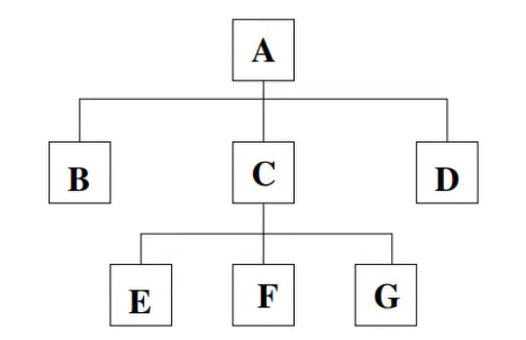
\includegraphics[width=0.3\linewidth]{Degree//static/ST_module_heirarchy.png}
        \caption{Module Hierarchy}
        \label{fig:ST-module-heirarchy}
    \end{figure}
\end{itemize}

\subsection{Design Integration Testing}
\begin{itemize}
    \item Graph models for integration testing are called \textbf{Call graphs}.
    \item For graph models, nodes now become modules/test stubs/test drivers and edges become interfaces.
    \item \textbf{Structural coverage criteria}: Deals with calls over interfaces.
    \item \textbf{Data flow coverage criteria}: Deals with exchange of data over interfaces.
    \item Node coverage will be to call every module at least once.
    \item Edge coverage is to execute every call at least once.
    \item Specified path coverage can be used to test a sequence of method calls.
    \item Data flow interfaces among modules are more complicated than control flow interfaces.
    \item \textbf{Caller}: A module that invokes/calls another module.
    \item \textbf{Callee}: The module that is called.
    \item \textbf{Call site}: The statement or node where the call appears in the code.
    \item \textbf{Actual parameters}: Variables in the caller.
    \item \textbf{Formal parameters}: Variables in the callee.
    \item \textbf{Coupling variables} are variables that are defined in one unit and used in the other.
    \item \textbf{Parameter coupling}: Parameters are passed in calls.
    \item \textbf{Shared data coupling}: Two units access the same data through global or shared variables.
    \item \textbf{External device coupling}: Two units access an external object like a file.
    \item \textbf{Message-passing interfaces}: Two units communicate by sending and/or receiving messages over buffers/channels.
    \item Since focus is on testing interfaces, we consider the \textbf{last definitions} of variables before calls to and returns from the called units and the \textbf{first uses} inside the modules and after calls.
    \item \textbf{Last-def}: The set of nodes that define a variable $x$ and has a def-clear path from the node through a call site to a use in the other module. Can be in either direction.
    \item \textbf{First-use}: The set of nodes that have uses of a variable $y$ and for which there is a def-clear and use-clear path from the call site to the nodes.
    \item A \textbf{coupling du-path} is from a last-def to a first-use.
    \item \textbf{All-coupling-def coverage}: A path is to be executed from every last-def to at least one first-use.
    \item \textbf{All-coupling-use coverage}: A path is to be executed from every last-def to every first-use.
    \item \textbf{All-coupling-Du-paths coverage}: Every simple path from every last-def to every first-use needs to be executed.
    \item The above criteria can be met with side trips.
    \item Only variables that are used or defined in the callee are considered for du-pairs and criteria.
    \item \textbf{Transitive du-pairs} (A calls B, B calls C and there is a variable defined in A and used in C) is not supported in this analysis.
\end{itemize}

\section{Specification Testing}
\subsection{Sequencing Constraints}
\begin{itemize}
    \item A \textbf{design specification} describes aspects of what behavior a software should exhibit. Behaviour exhibited by software need not mean the implementation directly. It could be a \textbf{model} of the implementation.
    \item For testing with graphs, we consider two types of design specifications. \textbf{Sequencing constraints} on methods/functions, and \textbf{State behavior} descriptions of software.
    \item \textbf{Sequencing constraints} are rules that impose constraints on the order in which methods may be called.
    \item Typically encoded as preconditions or other specifications. They may or may not be given as a part of the specification or design.
    \item Consider the example of a simple Queue, a precondition can be that at least one element must be on the queue before removing and a postcondition can be that $e$ is on the end of the queue to enqueue $e$.
    \item Simple sequencing constraint: enqueue must be called before dequeue.
    \item This does not include the requirement that we must have at least as many enqueue calls as dequeue calls. Need \textit{memory} which can be captured in the \textit{state} of the queue as the application code executes.
    \item Absence of sequencing constraints usually indicates more faults.
\end{itemize}

\subsection{Finite State Machines}
\begin{itemize}
    \item A \textbf{Finite State Machine} is a graph that describes how software variables are modified during execution.
    \item Nodes: \textbf{States}, representing sets of values for (key) variables.
    \item Edges: \textbf{Transitions}, which model possible changes from one state to another. Transitions have \textbf{guards} and/or \textbf{actions} associated with them.
    \item FSMs can model many kinds of systems like embedded software, abstract data types, hardware circuits etc.
    \item Creating FSM models for design helps in precise modelling and early detection of errors through analysis of the model.
    \item Many modelling notations support FSMs: Unified Modeling Language(UML), state tables, Boolean logic.
    \item FSMs are good for modelling control intensive applications not ideal for modelling data intensive applications.
    \item FSMs can be annotated with different types of \textbf{actions}: Actions on transitions, Entry actions to nodes, Exit actions on nodes.
    \item Actions can express changes to variables or conditions on variables.
    \item \textbf{Preconditions (guards)}: Conditions that must be true for transition to be taken.
    \item \textbf{Triggering events}: Changes to variables that cause transitions to be taken.
    \item Node coverage: Execute every state(state coverage).
    \item Edge coverage: Execute every transition(transition coverage).
    \item Edge-pair coverage: Execute every pair of transitions(transition-pair).
    \item Control flow graphs are \textbf{not} FSMs representing software/codes.
    \item Call graphs are also \textbf{not} FSMs representing software/codes.
    \item We need to consider values of variables to represent states of FSMs and statements/actions that result in change of values of variables(states) result in transitions.
\end{itemize}

\section{Testing Source Code: Classical Coverage Criteria}
\begin{itemize}
    \item The most common graph model for source code is control flow graph.
    \item Structural coverage criteria over control flow graphs deal with \textbf{covering} the code in some way or other.
    \item Data flow graphs augments the control flow with data.
    \item \textbf{Code coverage}: Statement coverage, branch coverage, decision coverage, Modified Condition Decision Coverage(MCDC), path coverage etc.
    \item Node coverage is same as statement coverage, edge coverage is same as branch, and prime path coverage is the same as loop coverage.
    \item \textbf{Cyclomatic complexity}: Basis path testing, structural testing. It is a software metric used to indicate the (structural) complexity of a program.
    \item Cyclomatic complexity represents the number of \textbf{linearly independent paths} in the control flow graph of a program.
    \item \textbf{Basis path testing} deals with testing each linearly independent path in the CFG of the program.
    \item A \textbf{linearly independent path} of execution in the CFG of a program is a path that does not contain other paths within it. This is very similar to prime paths, every linearly independent path is a prime path.
    \item The cyclomatic complexity $M=E-N+2P$, where $E$ is the number of edges, $N$ is the number of nodes, and $P$ is the number of connected components.
    \item When graph correspond to a single program, $M=E-N+2$.
    \item Another way of measuring cyclomatic complexity is to consider \textit{strongly connected components} in CFG. Can be obtained by connecting the final node back to the initial node. Cyclomatic complexity obtained this way is popularly called as \textbf{cyclomatic number}.
    \item If it is less than 10 then the code is not too complex.
    \item \textbf{Data flow testing}: Data flow coverage.
    \item \textbf{Decision-to-decision path} is a path of execution between two decisions in the CFG.
    \item A \textbf{chain} is a path in which initial and terminal vertices are distinct. All the interior vertices have both in-degree and out-degree as 1.
    \item A \textbf{maximal chain} is a chain that is not a part of any other.
    \item A \textbf{DD-path} is a set of vertices in the CFG that satisfies one of the following conditions:
    \begin{enumerate}
        \item It consists of a single vertex with in-degree 0(initial vertex).
        \item It consists of a single vertex with out-degree 0(terminal vertex).
        \item It consists of a single vertex with in-degree $\geq 2$ or out-degree $\geq 2$(decision vertices).
        \item It consists of a single vertex with in-degree and out-degree as 1.
        \item It is a maximal chain of length $\geq 1$.
    \end{enumerate}
    \begin{figure}[H]
        \centering
        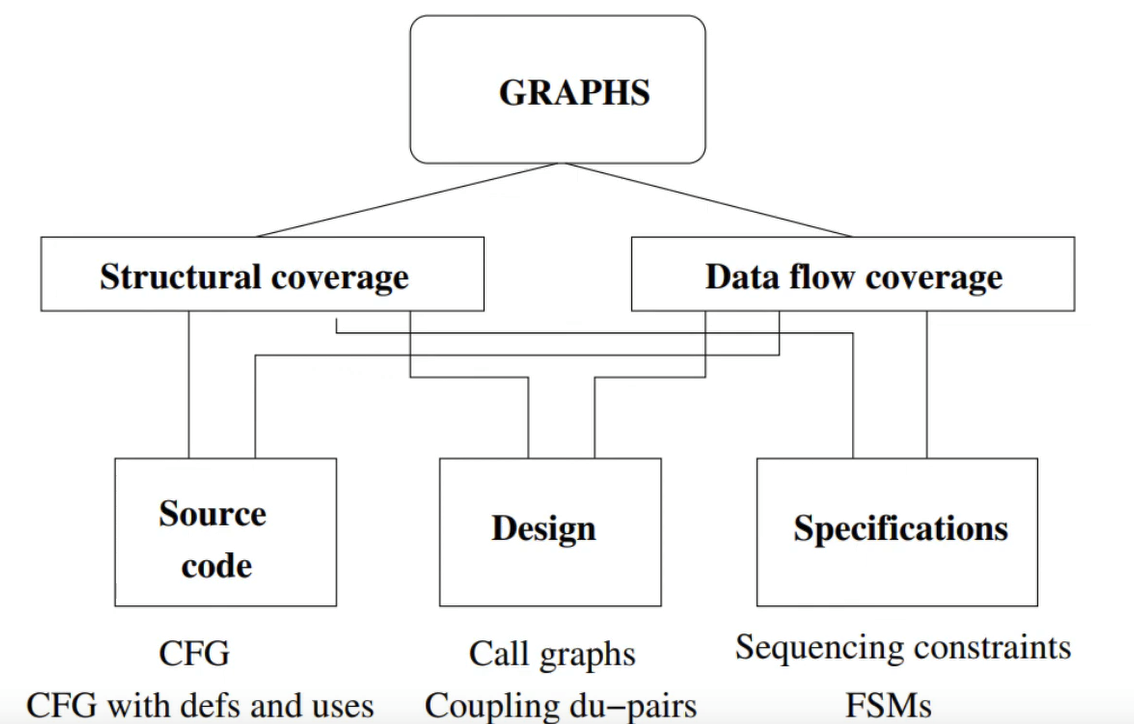
\includegraphics[width=0.5\linewidth]{Degree//static/ST_Graph_summary.png}
        \caption{Graph Coverage Criteria Summary}
        \label{fig:ST-graph-coverage-summary}
    \end{figure}
\end{itemize}

\section{Logic Based Testing}
\subsection{Basics}
\begin{itemize}
    \item The fragment of logic that we consider is popularly known as \textbf{predicate logic} or \textbf{first order logic}.
    \item An \textbf{atomic proposition} is a term that is either \textbf{true} or \textbf{false}.
    \item Propositional logic deals with combining propositions using \textbf{logical connectives} to form \textbf{formulas} which are complicated statements.
    \item Common logical connectives used in proportional logic are
    \begin{enumerate}
        \item $\lor$ Disjunction
        \item $\land$ conjunction
        \item $\neg$ negation
        \item $\supset$ or $\implies$ implies
        \item $\equiv$ or $\iff$ equivalence
    \end{enumerate}
    \item The set $\phi$ of formulas of propositional logic is the smallest set satisfying the following conditions
    \begin{enumerate}
        \item All atomic propositions is a member of $\phi$
        \item If $\alpha$ is a member of $\phi$, so is $\neg \alpha$
        \item If $\alpha$ and $\beta$ are members of $\phi$ so is $\alpha \lor \beta$
    \end{enumerate}
    \item Truth tables are a simple way of calculating the semantics of a given propositional logic formula.
    \item We \textit{split} a formula into its \textbf{sub-formulas} repeatedly till we \textit{reach} propositions.
    \item A formula $\alpha$ is said to be \textbf{satisfiable} if there exists a valuation $v$ such that $v(\alpha)=T$.
    \item A formula of $\alpha$ is to be \textbf{valid} or is called a \textbf{tautology} if for every valuation it gives True.
    \item A formula of $\alpha$ is said to be a \textbf{contradiction} if for every valuation it gives False.
    \item Atomic propositions in propositional logic are just like variables that are of type \textbf{Boolean}.
    \item A \textbf{predicate} is an expression that evaluates to a Boolean value.
    \item A \textbf{clause} is a predicate that does not contain any logical operators.
\end{itemize}

\subsection{Coverage Criteria}
\begin{itemize}
    \item Let $P$ be a set of predicates and $C$ be a set of clauses in the predicates in $P$.
    \item For each predicate $p\in P$, let $C_p$ be the clauses in $p$. $C_p\{c|c\in p\}$
    \item \textbf{Predicate Coverage}: For each $p\in P$, TR contains two requirements: $p$ evaluates to true and $p$ evaluates to false. For a set of predicates associated with branches, predicate coverage is the same as edge coverage.
    \item \textbf{Clause Coverage}: For each $c\in C$, TR contains two requirements: $c$ evaluates to true and $c$ evaluates to false. Clause coverage \textbf{does not} subsume predicate coverage.
    \item \textbf{Combinatorial Coverage}: For each $p\in P$, TR contains test requirements for the clauses in $C_p$ to evaluate to each possible combination of truth values. Commonly called as \textbf{multiple condition coverage}.
    \item Combinatorial coverage in many times not feasible.
    \item Sometimes, the truth of certain clauses in predicate makes the other clauses non-influential on the predicate.
    \item At a given point in time, we are interested in one clause in a predicate, we call this the \textbf{major clause}. All other clauses are \textbf{minor clauses}.
    \item  Given a major clause $c_i$ in predicate $p$, we say that $c$ \textbf{determines} $p$ if the minor clauses $c_j\in C_p$, $j\neq i$, have values so that changing the truth values of $c_i$ changes the truth value of $p$. 
    \item \textbf{Active Clause Coverage}: For each $p\in P$ and each major clause $c_i\in C_p$, choose minor clauses $c_j, j\neq i$, so that $c_i$ determines $p$. TR has requirements for each clause as a major clause. For a predicate with $n$ clauses, $n+1$ distinct test requirements suffice to achieve clause coverage.
    \item \textbf{Modified Condition Decision Coverage(MCDC)} is the same as Active Clause Coverage.
    \item \textbf{General Active Clause Coverage}: TR has two requirements for each $c_i$, $c_i$ evaluates to true and evaluates to false. The values chosen for the minor clauses $c_j$ do not need to be the same when $c_i$ is true as when $c_i$ is false. GACC \textbf{does not} subsume predicate coverage.
    \item \textbf{Correlated Active Clause Coverage}: The values chosen for minor clauses $c_j$ must cause $p$ to be true for one value of the major clause $c_i$ and false for the other. CACC subsumes predicate coverage.
    \item \textbf{Restricted Active Clause Coverage}: The values chosen for the minor clauses $c_j$ must be the same when $c_i$ is true and when it is false.
    \item \textbf{Inactive Clause Coverage}: For each $p\in P$ and each major clause $c_i\in C_p$, choose minor clauses $c_j, j\neq i$ so that $c_i$ does not determine $p$. TR now has four requirements for $c_i$, $p$ is true/false for $c_i$ true/false.
    \item \textbf{General Inactive Clause Coverage}: The values chosen for the minor clauses $c_j$ may vary amongst the four cases.
    \item \textbf{Restricted Inactive Clause Coverage}: The values chosen for the minor clauses $c_j$ must be the same for same values of $p$.
    \begin{figure}[H]
        \centering
        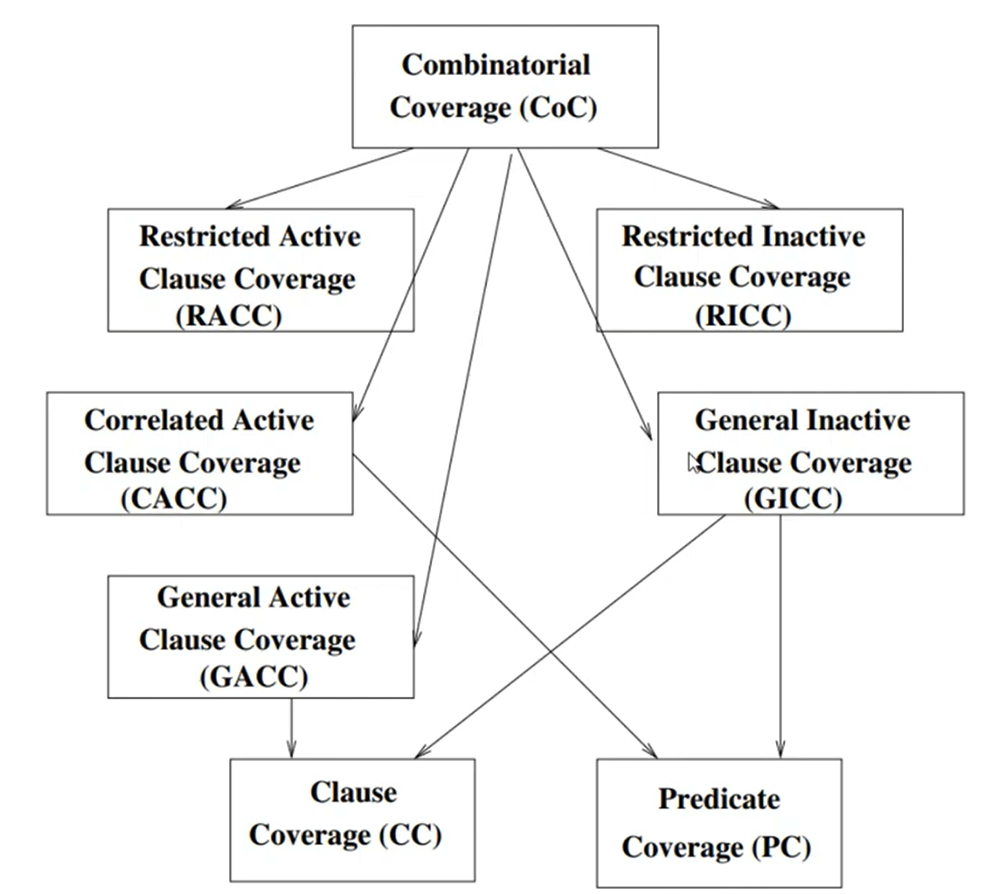
\includegraphics[width=0.5\linewidth]{Degree//static/ST_logic_subsume_summary.png}
        \caption{Logic Coverage Criteria Subsumption Summary}
    \end{figure}
    \item As long as a predicate or a clause is not valid/not a contradiction, we can find test cases to achieve predicate and clause coverage.
    \item Need to identify the \textbf{correct} predicates and pass them to a \textbf{SAT/SMT solver} to check if the predicate is \textbf{satisfiable}.
    \item Making a clause determine a predicate
    \begin{enumerate}
        \item Consider a predicate $p$ with a major clause $c$
        \item Let $p_{c=true}$ represent the predicate $p$ with every occurrence of $c$ replaced with $true$, and $p_{c=false}$.
        \item Note that neither $p_{c=true}$ nor $p_{c=false}$ contains any occurrence of $c$.
        \item Define $p_c=p_{c=true}\oplus p_{c=false}$, $\oplus$ represents the exclusive or operator.
        \item $p_c$ describes the exact conditions under which the value of $c$.
        \item If $p_c$ is true then $c$ determines $p$(ACC) and if $p_c$ is false then $p$ is independent of $c$(ICC).
    \end{enumerate}
    \item For a predicate $p$ where the value of $p_c$ for a clause $c$ turns out to be true, then ICC criteria are infeasible with respect to $c$. Similarly, if $p_c$ turns out to be false, ACC criteria are infeasible.
    \item Site to test coverage criteria can be found \href{https://cs.gmu.edu:8443/offutt/coverage/LogicCoverage}{here}.
\end{itemize}

\subsection{Applied to Test Specification}
\begin{itemize}
    \item Specifications can be written in a formal language or in English. They include several logical conditions.
    \item Pre-conditions, post-conditions and assertions that occur in code and invariant properties about loops contain several logical predicates.
    \item Programmers often include preconditions for their methods. Often expressed as comments in method headers.
    \item A predicate is in \textbf{Conjunctive Normal Form} (CNF) if it consists of clauses or disjuncts connected by the conjunction (and) operator. Example: $(a\lor b)\land(c\lor d)$.
    \item ACC test requirements is all \textit{true} and then a \textit{diagonal} of false values.
    \item \textbf{Predicate Coverage}: All clauses need to be true for the true case and at least one clause needs to be false for the false case. 
    \item \textbf{Clause coverage}: Needs all clauses to be true or false.
    \item For ACC criteria, each minor clause is true and for remaining tests, each clause is made to be false in turn.
    \item A predicate is in \textbf{Disjunctive Normal Form} (DNF) if it consists of clauses or conjuncts connected by th disjunction (or) operator. Example: $(a\land b)\lor(c\land d)$.
    \item ACC test requirements is all \textit{false} and then a \textit{diagonal} of true values.
\end{itemize}

\subsection{Applied to Finite State Machine}
\begin{itemize}
    \item Test cases for various test requirements need inputs and expected outputs.
    \item Inputs could be states from which transitions originate or actions that result in transitions.
    \item Outputs could be states resulting from transitions and actions associated with the resulting states, if any.
    \item These need to be derived from the FSMs.
\end{itemize}

\subsection{SMT Solvers}
\begin{itemize}
    \item The \textbf{satisfiability problem (SAT)}, also called the Boolean satisfiability problems or the propositional satisfiability problem is the problem of determining if there exists an assignment of True/False values that \textbf{satisfies} a given propositional logic.
    \item A satisfying assignment is an assignment of True/False values to the atomic propositions such that the formula evaluates to true.
    \item SAT is the first problem that was proven to be NP-complete.
    \item Currently, there is no known algorithm that efficiently solves each instance of the SAT problem.
    \item The tools that solve such instances are referred to as \textbf{SAT Solvers}.
    \item There are a few well-known techniques that they implement to find solutions, some are good at proving unsatisfiability.
    \item Satisfiability problem of general first order logic is \textit{undecidable}, i.e., there are \textit{no} algorithms that will take every instance of a predicate logic formula and report whether it is satisfiable or not.
    \item \textbf{Satisfiability Modulo Theories (SMT)} is the problem of determining whether a given predicate (or a formula) is satisfiable.
    \item \textbf{SMT solvers} are tools that work towards solving the SMT problem for a simpler, often practical, subset of the logic.
    \item SMT solvers are used extensively in formal verification and program analysis, for proving the \textit{correctness} of programs.
\end{itemize}

\subsection{Symbolic Testing}
\begin{itemize}
    \item \textbf{Symbolic execution} is a means of analyzing a given program to determine what inputs cause each part of the program to execute. This can be effectively used for exercising different executions of the program.
    \item Consider the following program, and it's respective symbolic execution
    \begin{figure}[H]
        \centering
        \begin{subfigure}[b]{0.20\textwidth}
            \centering
            \begin{verbatim}
    Sum(a,b,c){
        x = a + b;
        y = b + c;
        z = (x+y) - b;
        return z
    }
            \end{verbatim}
            \caption{Sum of three numbers}
        \end{subfigure}
        \hfill
        \begin{subfigure}[b]{0.70\textwidth}
            \begin{tabular}{||l|c|c|c|c|c|c|c||}
                \hline
               After statement  & $x$ & $y$ & $y$ & $a$ & $b$ & $c$ & PC \\
               \hline
               1 & ? & ? & ? & $\alpha_1$ & $\alpha_2$ & $\alpha_3$ & true \\
               2 & $\alpha_1+\alpha_2$ & - & - & - & - & - & -\\
               3 & - & $\alpha_2+\alpha_3$ & - & - & - & - & -\\
               4 & - & - & $\alpha_1+\alpha_2+\alpha_3$ & - & - & - & -\\
               \cline{2-8}
               5 & \multicolumn{7}{c||}{Returns $\alpha_1+\alpha_2+\alpha_3$}\\
               \hline
            \end{tabular}
            \caption{Symbolic Execution Table}
        \end{subfigure}
        \caption{Symbolic Execution Example}
        \label{fig:enter-label}
    \end{figure}
    \item PC is the Path condition/constraint
    \item Instead of concrete expression, use symbolic expression.
    \item During execution, collect path conditions and solve them symbolically.
    \item Now we can use constraint solver to get concrete values such that all path constraints are true and false.
    \item \textbf{Program proving} involves proving programs correct. Program proving involves formal methods.
    \item It is used to prove absence of errors.
    \item Three techniques: Model checking, Theorem proving, and Program analysis.
    \item Symbolic testing uses program analysis.
    \item Symbolic execution is a practical approach between the two extremes of program testing and proving.
    \item Program variables are represented as symbolic expressions over the symbolic input values.
    \item Symbolic state $\sigma$ maps variables to symbolic expressions.
    \item Symbolic path constraints, PC, is a quantifier-free, first order formula over symbolic expressions.
    \item All the execution paths of a program can be represented using a tree, called the \textbf{execution tree}.
    \item Symbolic execution is used to generate a test input for each execution path of a program.
    \item At the beginning of symbolic execution: $\sigma$ is initialized to an empty map.
    \item At a read statement: symbolic execution adds the mapping assigning the variable being read to its new symbolic variable, to $\sigma$
    \item At every assignment, $v=e$: symbolic execution updates $\sigma$ by mapping $v$ to $\sigma(e)$, the symbolic expression obtained by evaluating $e$ in the current symbolic state.
    \item At the beginning of execution: PC is initialized to true
    \item At a conditional statement $if(e)$ then $S_1$ else $S_2$: PC is updated to $PC\land \sigma(e)$("then" branch) and a fresh path constraint PC' is created and initialized to $PC\land \lnot \sigma(e)$("else" branch).
    \item If PC (PC') is satisfiable for some assignment of concrete to symbolic values, then symbolic execution continues along the "then" ("else") branch with $\sigma$ and PC (PC').
    \item If any of PC or PC' is not satisfiable, symbolic execution terminates along the corresponding path.
    \item At the end of symbolic execution along an execution path of the program, PC is solved using a constraint solver to generate concrete input values.
    \item Execution can also be terminated if the program hits an exit statement or an error.
    \item Consider an infinite while loop with condition $N>0$, PC for the loop with a sequence of $n$ true-s followed by a false is
    \begin{equation*}
        (\land_{i\in [1,n]}N_i>0)\land (N_{n+1}\leq 0)
    \end{equation*}
    where each $N_i$ is a fresh symbolic value.
    \item In general, symbolic execution of code containing loops or recursion may result in an infinite number of paths if the termination condition for the loop or recursion is symbolic.
    \item In practice, one needs to put a limit on the search, a timeout, or a limit on the number of paths, loop iterations or exploration depth.
    \item Symbolic testing is dependent on a constraint solver that takes a path constraint and gives a set of input values to be used as test cases.
    \item These input values are solutions to the path constraint, popularly known as the satisfiability problem.
\end{itemize}

\subsection{Concolic Testing}
\begin{itemize}
    \item Concolic testing performs symbolic execution dynamically, while the program is executed on some concrete inputs.
    \item Concolic: Concrete $+$ Symbolic
    \item Maintains a concrete state and a symbolic state
    \item Whenever symbolic execution is not possible, then it does normal execution of the program.
    \item Generate random input, execute program on random input.
    \item Collect symbolic path constraints encountered along this execution.
    \item Steer program execution along different execution paths
    \begin{enumerate}
        \item Use constraint solver to infer variants of symbolic path constraints.
        \item Generate inputs that drive program along different execution paths
        \item Repeat till all execution paths are explored/user-defined coverage criteria is met or time budget expires.
    \end{enumerate}
    \item \textbf{Note}: Understanding DART is very confusing, don't spend too much time on this.
    \item Directed Automated Random Testing is a testing technique that applies to the unit testing phase in software development. Can be applied to large programs, where typically random testing is done.
    \item DART is a concolic testing tool.
    \item DART combines three main techniques in order to automate unit testing of programs
    \begin{enumerate}
        \item Automated extraction of the interface of a program with its external environment using static source-code parsing.
        \item Automatic generation of a test driver for this interface that performs random testing to simulate the most general environment the program can operate in, and
        \item Dynamic analysis of how the program behaves under random testing and automatic generation of new test inputs to direct systematically the execution along alternative program paths.
    \end{enumerate}
    \item DART dynamically gathers knowledge about the execution of the program, called directed search.
    \item \textbf{Memory} $\mathcal{M}$: a mapping from memory address $m$ to say $32$-bit words.\\
    $+$ denotes updating of memory. For example, $\mathcal{M}':=\mathcal{M}+[m\to v]$
    \item \textbf{Symbolic variables} are identified by their addresses.
    \item In an expression, $m$ denotes either a memory address or the symbolic variable identified by address $m$, depending on the context.
    \item A \textbf{symbolic expression}, $e$ is given by $m$, $c$(a constant), $\ast(e,e')$(multiplication), $\leq (e,e')$(comparison), $\lnot e'$(negation), $\ast e'$(pointer dereference) etc.
    \item Symbolic variables of an expression $e$ are the set of addresses $m$ that occur in it.
    \item Expressions have no side effects.
    \item For DART, we need to define semantics of a program at memory level.
    \item At memory level, statements are specifically tailored abstractions of the machine instructions that are actually executed.
    \item Statement labels: A set of labels that denote instruction addresses.
    \item If $l$ is the address of a statement other than abort or halt then $l+1$ is also an address of a statement. There is an initial address, say $l_0$.
    \item A function statement at $(I,\mathcal{M})$ specifies the next statement to be executed.
    \item Let $C$ be the set of conditional statements and $A$ be the set of assignment statements in $P$
    \item A program execution $w$ is a finite sequence of Execs $=(A\cup C)\ast (abort|halt)$
    \item A further simplifies program execution: $w$ is of the form $\alpha_1c_1\alpha_2c_2...c_k\alpha_{k+1}s$ where $\alpha_i\in A^*$, $c_i\in C$, and $s\in \{abort, halt\}$.
    \item An alternate view: Consider Execs(P) is a tree; assignment nodes have one or two successors, leaves are labeled by abort or halt.
    \item Each input vector results as an execution sequence, as a path in this tree.
    \item DART maintains a symbolic memory $\mathcal{S}$ that maps memory addresses to expressions.
    \item While the main DART algorithm runs, it will evaluate the symbolic path constraints using this algorithm and solve the path constraints to generate directed test cases.
    \item To start with, $\mathcal{S}$ just maps each $m\in M_o$ to itself.
    \item The mapping $\mathcal{S}$ is completed by evaluating expressions symbolically.
    \item When unsolvable path constraints are encountered, the algorithm uses concrete values instead of symbolic values.
\end{itemize}

\section{Black Box Testing}
\subsection{Requirements}
\begin{itemize}
    \item \textbf{Requirement}: A condition or capability needed by a stakeholder to solve a problem or achieve an objective.
    \item \textbf{Product requirements}: Describe the properties of a product or a system. The product can be a software product too.
    \item \textbf{Process requirements}: Describe the activities to be done by the organization involved in the product development.
    \item \textbf{Business requirements}: Specifies characteristics from the view point of a user or a stakeholder. Document: StRS, Stakeholder Requirements Specification.
    \item \textbf{User requirements}: Specifies what the user expects the software to be able to do. Document: URS, User Requirements Specification. A mutually agreed contract details what the software must do from the point of view of a user.
    \item \textbf{Functional requirements}: Defines a function of a system or its component, where a function is described as a specification of behavior between inputs and outputs. Describes specific/particular results/behaviour of a system. Can be given as use cases. Document: FRS, Functional Requirements Specification. Design document caters to functional requirements.
    \item \textbf{Non-functional requirements}: Specifies criteria that can be used to judge the operation of a system, rather than specific behaviors. Define how a system is supposed to be. Specified as different quality parameters.
    \item \textbf{Regulatory requirements}: Regulation is the management of systems/software as per a set of rules and regulations, specific to several different factors including the environment, business, safety etc. Regulatory requirements could differ from one country to another.
    \item \textbf{Black Box testing}: Black-box testing deals with requirements and spans most of the requirements sketched above. Treats the executable artifacts (code) as a black box. Test cases are designed purely based on the requirements to be tested, inputs and outputs.
\end{itemize}

\subsection{Functional Testing}
\begin{itemize}
    \item A program $P$ is viewed as a function transforming inputs to outputs. Given inputs $x_i$, $P$ computes outputs $y_i$ such that $y_i = P(x_i)$.
    \item Precisely identify the domain of each input and each output variable.
    \item Select values from the data domain of each variable having important properties.
    \item Consider combinations of special values from different input domains to design test cases.
    \item Consider input values such that the program under test produces special values from the domains of the output variables.
    \item Even though functional testing is a black-box testing technique, sometimes, we need to know minimal context information to get relevant values for inputs and outputs.
    \item \textbf{Equivalence class Partitioning}: If the input domain is too large for all its elements to be used as test cases, the input domain is partitioned into a finite number of subdomains for selecting test inputs.
    \item Each subdomain is known as an equivalence class.
    \item One subdomain serves as a source for selecting one test input, any one input from each domain is good enough.
    \item All inputs from one subdomain have the same effect in the program, output will be the same.
    \item \textbf{Boundary Value Analysis} is about selecting test inputs near the boundary of a data domain so that the data both within and outside an equivalence class are selected.
    \item BVA produces test inputs near the boundaries to find failures caused by incorrect implementation at the boundaries.
    \item Once equivalence class partitions the inputs, boundary values are chosen on and around the boundaries of the partitions to generate test input for BVA.
    \item Programmers often make mistakes at boundary values and hence BVA helps to test around the boundaries.
    \item The partition specifies a range: Construct test cases by considering the boundary points of the range and the points just beyond the boundaries of the range.
    \item The partition specifies a number of values: Construct test cases for the minimum and the maximum value of the number. In addition, select a value smaller than the minimum and a value larger than the maximum.
    \item The partition specifies an ordered set: Consider the first and last elements of the set.
    \item \textbf{Decision tables} handle multiple inputs by considering different combinations of equivalence classes. Very popular to test several different categories of software.
    \begin{table}[H]
        \centering
        \begin{tabular}{cccccccccc}
            \hline
              & & \multicolumn{8}{c}{Rules or Combinations}\\
             \hline
            Conditions & Values & $R_1$ & $R_2$ & $R_3$ & $R_4$ & $R_5$ & $R_6$ & $R_7$ & $R_8$\\
            \hline
            $C_1$ & $Y,N,-$ & $Y$ & $Y$ & $Y$ & $Y$ & $N$ & $N$ & $N$ & $N$\\
            $C_2$ & $Y,N,-$ & $Y$ & $Y$ & $N$ & $N$ & $Y$ & $Y$ & $N$ & $N$\\
            $C_3$ & $Y,N,-$ & $Y$ & $N$ & $Y$ & $N$ & $Y$ & $N$ & $Y$ & $N$\\
            Effects & \multicolumn{9}{c}{}\\
            $E_1$ & & 1 & & 2 & 1 & & & & \\
            $E_2$ & & & 2 & 1 & & & 2 & 1 & \\
            $E_3$ & & 2 & 1 & 3 & & 1 & 1 & & \\
            \hline
        \end{tabular}
        \caption{Decision Table example}
    \end{table}
    \item A decision table has
    \begin{enumerate}
        \item A set of conditions and a set of effects arranged in a column. Each condition has possible value (yes (Y), no(N), don’t care(–)) in the second column.
        \item For each combination of the three conditions there are a set of rules from R1 to R8. Each rule has a Y/N/– response and contains an associated set of effects (E1, E2 and E3).
        \item For each effect, an effect sequence number specifies the order in which the effect should be carried out if the associated set of conditions are satisfied.
    \end{enumerate}
    \item In \textbf{random testing}, test inputs are selected randomly from the input domain.
\end{itemize}

\subsection{Input Space Partitioning}
\begin{itemize}
    \item Given a set $S$, a partition of $S$ is a set $\{S_1,S_2,...,S_n\}$ of subsets of $S$ such that\\
    The subsets $S_i$ of $S$ are pair-wise disjoint, $S_i\cap S_j=\phi$.\\
    The union of the subsets $S_i$ is the entire set $S$, $\bigcup_iS_i=S$.
    \item The set that is split into partitions while doing testing is the input domain.
    \item Input domain can be several different sets, one for each input. We may or may not consider all the inputs while doing partitioning.
    \item Each partition represents one characteristic of the input domain, the program under test will behave in the same way for any element from the partitions.
    \item There is an underlying equivalence relation that influences the partitions, so input space partitioning is popularly known as equivalence partitioning.
    \item Each partition is based on some characteristic of the program $P$ that is being tested.
    \item Characteristics that define partitions must ensure that the partition satisfies two properties: \textbf{completeness} (The partitions must cover the entire domain) and \textbf{disjoint} (The partitions must not overlap).
    \item The following are the steps in input domain modelling.
    \begin{enumerate}
        \item Identification of testable functions.
        \item Identify all the parameters that can affect the behaviour of a given testable function. These parameters together form the input domain of the function under test.
        \item Modelling of the input domain identified in the previous step: Identify the characteristics and partition for each characteristic.
        \item Get the test inputs: A test input is a tuple of values, one for each parameter. The test input should belong to exactly one block from each characteristic.
    \end{enumerate}
    \item Input domain can be modelled in several different ways, needs extensive knowledge of the domain. Both valid and invalid inputs need to be considered.
    \item \textbf{Interface-based modelling}: This method considers each parameter in isolation.
    \item \textbf{Strengths}: It is easy to identify the characteristics, hence easy to model the input domain.
    \item \textbf{Weaknesses}: Not all information that is available to the test engineer will be reflected in the interface domain model, the model can be incomplete.\\
    Some parts of the functionality may depend on the combinations of specific values of several interface parameters. Analyzing in isolation will miss the combinations.
    \item Characteristics in this approach are easy, directly based on the individual inputs. Inputs can be obtained from specifications.
    \item \textbf{Functionality based modelling}: This method identifies characteristics based on the overall functionality of the system/function under test, rather than using the actual interface.
    \item \textbf{Strengths}: There is a widespread belief that this approach yields better results than interface-based approach. This is based on the requirements, test case design can start early in the development lifecycle.
    \item \textbf{Weaknesses}: Since it is based on functionality, identifying characteristics is far from trivial. This makes test case design difficult.
    \item Pre-conditions, post-conditions are typical sources for identifying functionality-based characteristics. Implicit and explicit relationships between variables are another good source. Missing functionality is another characteristic. Domain knowledge is needed.
    \item \textbf{Valid values}: Include at least one set of valid values.
    \item \textbf{Sub-partitions}: A range of valid values can be further partitioned such that each sub-partition exercises a different part of the functionality.
    \item \textbf{Boundaries}: Include values at and close to the boundaries (BVA).
    \item \textbf{Invalid values}: Include at least one set of invalid values.
    \item \textbf{Balance}: It might be cheap or free to add more partitions to characteristics that have fewer partitions.
    \item \textbf{Missing partitions}: Union of all the partitions should be the complete input space for that characteristic.
    \item \textbf{Overlapping partitions}: There should be no overlapping partitions.
    \item Typically, input domain has several different inputs, each of which can be partitioned.
    \item Each input domain can be partitioned in several different ways.
    \item For interface-based ISP, inputs are considered separately.
    \item For functionality-based ISP, input combinations cutting across partitions need to be considered.
    \item \textbf{All Combinations Coverage (ACoC)}: All combinations of blocks from all characteristics must be used. If we have three partitions as $[A,B]$, $[1,2,3]$ and $[x,y]$, then ACoC will have twelve tests.
    \item A test suite for ACoC will have a unique test for each combination.
    \item Total number of tests will be $\prod_{i=1}^nB_i$, $B_i$ is the number of blocks for each partition, $n$ is the number of partitions.
    \item ACoC is just an exhaustive testing of considering all possible partitions of the input domain and testing each combination of partitions.
    \item Apart from the partitions themselves, ACoC has no other advantages, it is like exhaustive testing with respect to the partitions.
    \item ACoC might not be necessary all the time.
    \item \textbf{Each Choice Coverage (ECC)}: One value from each block for each characteristic must be used in at least one test case.
    \item If the program under test has $n$ parameters $q_1,q_2,...,q_n$, and each parameter $q_i$ has $B_i$ blocks, then, a test suite for ECC will have at least $\max_iB_i$ values.
    \item ECC is a weak criterion.
    \item ECC will not be effective for arbitrary choice of test values.
    \item \textbf{Pair-Wise Coverage (PWC)}: A value from each block for each characteristic must be combined with a value from every block for each other characteristic.
    \item A test suite that satisfies PWC will pair each value with each other value or have at least $(\max_iB_i)^2$ values.
    \item \textbf{T-Wise Coverage (TWC)}: A value from each block for each group of $t$ characteristics must be combined.
    \item If the value for $T$ is chosen to be the number of partitions, then TWC is the same as ACoC.
    \item A test suite that satisfies TWC will have at least $(\max_iB_i)^t$ values.
    \item TWC is expensive in terms of the number of tests, going beyond PWC is mostly not useful.
    \item ACoC considers all combinations, ECC considers each combination.
    \item PWC and TWC considers combinations blindly without regard for which values are being combined.
    \item \textbf{Base Choice Coverage (BCC)}: A base choice is chosen for each characteristic, and a base test is formed by using the base choice for each characteristic. Subsequent tests are chosen by holding all but one base choice constant and using each non-base choice in each other characteristic.
    \item A test suite that satisfies BCC will have one base test, plus one test for each remaining block for each partition. Totally, $1+\sum_{i=1}^n(B_i-1)$.
    \item \textbf{Multiple Base Choices (MBCC)}: At least one, and possibly more, base choice blocks are chosen for each characteristic, and base tests are formed by using each base choice for each characteristic, at least once. Subsequent tests are chosen by holding all but one base choice constant for each base test and using each non-base choice in each other characteristic. The above coverage criteria will cover most of the different ways in which we can partition the inputs to test the software artifact.
    \item Assuming $m_i$ base choices for each characteristic and a total of $M$ base tests, MBCC requires $M+\sum_{i=1}^n(M\times (B_i-m_i))$ tests.
    \begin{figure}[H]
        \centering
        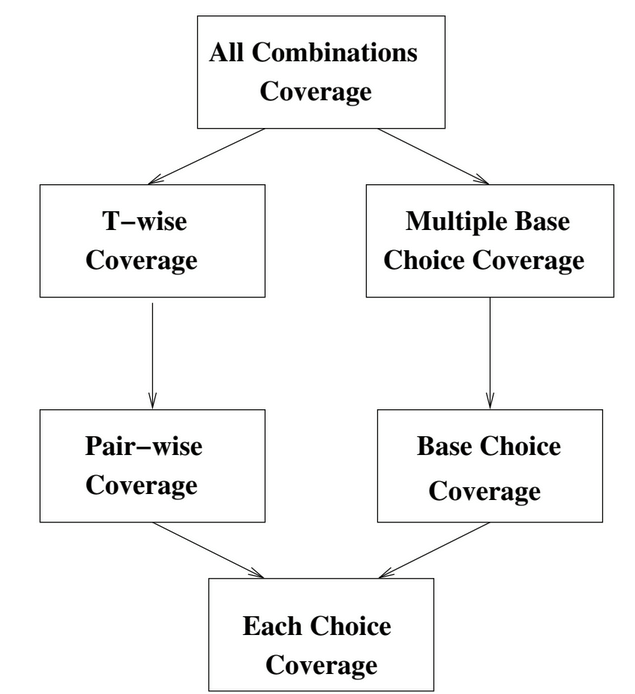
\includegraphics[width=0.35\linewidth]{Degree//static/ST_ISP_subsumption.png}
        \caption{ISP Subsumption relations}
    \end{figure}
    \item Some combinations of partitions can be infeasible in the input domain model.
    \item \textbf{Constraints} are relations between partitions from different characteristics.
    \item Two kinds of constraints
    \begin{enumerate}
        \item A block from one characteristic cannot be combined with a block from another characteristic.
        \item A block from one characteristic must be combined with a block from another characteristic.
    \end{enumerate}
    \item For ACoC, PWC and TWC, the only option is to drop the infeasible combinations from consideration.
    \item Constraints can be handled better with BCC and MBCC criteria. The base case(s) can be altered to handle infeasible constraints.
\end{itemize}

\section{Syntax Based Testing}
\subsection{Regular Expressions}
\begin{itemize}
    \item Syntax can be used to generate artifacts that are valid and those that are invalid.
    \item The structures/artifacts that we generate are sometimes test cases but, most of the time they are not. They are used to generate test cases.
    \item \textbf{Words}: The lexical level, defines how characters from tokens. Generally specified using \textbf{regular expressions}.
    \item \textbf{Phrases}: The grammar level, determines how tokens phrases. Generally specified using (deterministic) context-free grammars in \textbf{Backus-Naur form}.
    \item \textbf{Context}: Deals with types of variables, what they refer to etc. Generally specified using \textbf{context-sensitive grammars}.
    \item Syntax of regular expressions over an alphabet $A$
    \begin{equation*}
        r::=\phi \text{ }|\text{ } a\text{ }|\text{ } r+r\text{ }|\text{ }r\cdot r\text{ }|\text{ }r^*,\text{   where }a\in A
    \end{equation*}
    \item \textbf{Semantics}: Associates a language of words or strings, consider $L(r)\subseteq A^*$ with a regular expression $r$.
    \begin{equation*}
        \begin{split}
            L(\phi)&=\{\}\\
            L(a)&=\{a\}\\
            L(r+r')&=L(r)\cup L(r')\\
            L(r\cdot r')&=L(r)\cdot L(r')\\
            L(r^*)&=L(r)^*
        \end{split}
    \end{equation*}
    \item Consider expressions built from $a,b,\epsilon$, $\epsilon$ is a special empty word\\
    $(a^*+b^*)\cdot c$ are strings of only $a'$s or only $b'$s, followed by a $c$.
    \begin{figure}[H]
        \centering
        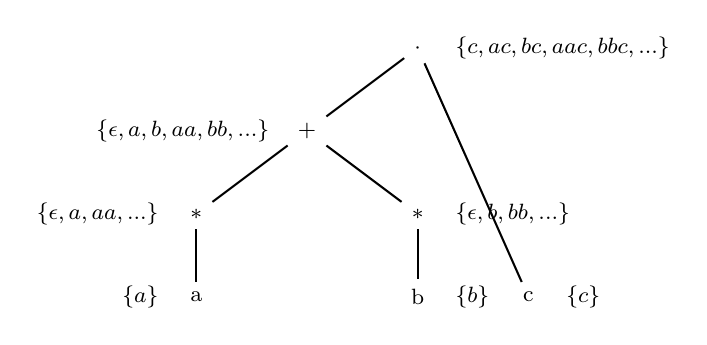
\begin{tikzpicture}[%
          sibling distance=8em,
          level distance=3em,
          edge from parent/.style={draw},
          every node/.style={font=\footnotesize}]
        
        % Root of the parse tree
        \node {$\cdot$}
          child { node {$+$}
            child { node {$*$}
              child { node {a} node[left=1em] {$\{a\}$} }
              node[left=1em] {$\{ \epsilon,a,aa,...\}$} 
            }
            child { node {$*$} 
                child {node {b} node[right=1em] {$\{b\}$} }
                node[right=1em] {$\{ \epsilon,b,bb,...\}$}
            }
            node[left=1em] {$\{ \epsilon,a,b,aa,bb,...\}$} 
          }
          child[level distance=9em] { node {c} node[right=1em] {$\{c\}$} }
          node[right=1em] {$\{ c,ac,bc,aac,bbc,...\}$} ;
        
        \end{tikzpicture}
        \caption{Parse Tree}
    \end{figure}
    $(a+b)^*abb(a+b)^*$ are strings that contain $abb$ as a sub-word\\
    $(a+b)^*b(a+b)(a+b)$ are strings that have third last letter as $b$.\\
    $(ab^*a)^*b^*$ are strings that optionally begin and end with an $a$, followed by a string of zero or more $b'$s.
    \item Context-Free Grammar example
    \begin{equation*}
        \begin{split}
            S&\to aX\\
            X&\to aX\\
            A&\to bX\\
            X&\to b
        \end{split}
    \end{equation*}
    Derivation of a string: Begin with $S$ and keep rewriting the current string by replacing a non-terminal by its RHS in a production of the grammar.\\
    Consider an example derivation
    \begin{equation*}
        S\implies aX\implies abX\implies abb
    \end{equation*}
    \item Language defined by $G$, written $L(G)$, is the set of all terminal string that can be generated by $G$.
    \item A \textbf{Context-Free Grammar (CFG)} is of the form
    \begin{equation*}
        G=(N,A,S,P)
    \end{equation*}
    where, $N$ is a finite set of non-terminal symbols\\
    $A$ is a finite set of terminal symbols\\
    $S\in N$ is the start non-terminal symbol\\
    $P$ is a finite subset of $N\times (N\cup A)^*$, called the set of productions or rules.
    \item $\alpha$ derives $\beta$ in $0$ or more steps: $\alpha\implies_G^*\beta$
    \item First define $\alpha \xrightarrow{n}\beta$ inductively
    \begin{enumerate}
        \item $\alpha \xrightarrow{1}\beta$ iff $\alpha$ is of the form $\alpha_1X\alpha_2$ and $X\to \gamma$ is a production in $P$, and $\beta=\alpha_1\gamma \alpha_2$
        \item $\alpha \xrightarrow{n+1}\beta$ iff there exists $\gamma$ such that $\alpha \xrightarrow{n}\gamma$ and $\gamma \xrightarrow{1}\beta$
    \end{enumerate}
    \item \textbf{Sentential form} of $G$: any $\alpha \in (N\cup A)^*$ such that $S\implies_G^*\alpha$
    \item Language defined by $G$
    \begin{equation*}
        L(G)=\{w\in A^*|S\implies_G^*w\}
    \end{equation*}
    \item $L\subseteq A^*$ is called \textbf{Context-Free Language (CFL)} if there is a CFG G such that $L=L(G)$
    \item \textbf{Note}: The above math is not that important, learn from the example.
    \item \textbf{Terminal Symbol Coverage (TSC)}: TR contains each terminal symbol $t$ in the grammar $G$.
    \item \textbf{Production Coverage (PC)}: TR contains each production $p$ in the grammar $G$.
    \item \textbf{Derivation Coverage (DC)}: TR contains every possible string that can be derived from the grammar $G$.
    \item PC subsumes TSC, if we cover every production, we cover every terminal.
    \item DC is an impractical/infeasible coverage criterion. The number of derivations is infinite for many useful grammars.
\end{itemize}

\subsection{Mutation Testing}
\begin{itemize}
    \item Mutation testing involves making syntactically valid changes to a software artifact and then testing the artifact.
    \item Grammars generate valid strings. We use derivations in grammars to generate invalid strings as well.
    \item Testing based on these valid and invalid strings is called \textbf{mutation testing}.
    \item \textbf{Ground string}: A string that is in the grammar.
    \item \textbf{Mutation operator}: A rule that specifies syntactic variations of strings generated from a grammer.
    \item \textbf{Mutant}: The result of one application of a mutation operator.
    \item For a given artifact, let $M$ be the set of mutants, each mutant $m\in M$ will lead to a test requirement.
    \item The testing goal in mutation testing is to kill the mutants by causing the mutant to produce a different output.
    \item Given a mutant $m\in M$ for a derivation $D$ and a test $t$, $t$ is said to kill $m$ iff the output of $t$ on $D$ is different from the output of $t$ on $m$.
    \item The derivation $D$ could be represented by the complete list of productions followed, or simply be the final string.
    \item \textbf{Mutation Coverage (MC)}: For each mutant $m\in M$, TR contains exactly one requirement, to kill $m$.
    \item the coverage in mutation equates to killing the mutants.
    \item the amount of coverage is usually written as a percent of mutants killed and is called \textbf{mutation score}.
    \item Higher mutation score doesn't mean more effective testing.
    \item When a grammar is mutated to produce invalid strings, the testing goal is to run the mutants to see if the behavior is correct.
    \item \textbf{Mutation Operator Coverage (MOC)}: For each mutation operator, TR contains exactly one requirement, to create a mutated string $m$ that is derived using the mutation operator.
    \item \textbf{Mutation Production Coverage (MPC)}: For each mutation operator, and each production that the operator can be applied to, TR contains the requirement to create a mutated string from that production.
    \item Exhausting mutation testing yields more requirements than other criteria.
    \item Mutation testing is difficult to apply by hand, automation is also complicated.
    \item \textbf{Program-based mutation}
    \begin{enumerate}
        \item Begin with the program (ground string).
        \item Apply one or more suitable mutation operators (mutant).
        \item Write tests to kill the mutant.
    \end{enumerate}
    \item \textbf{Stillborn mutant}: Mutants of a program result in invalid programs that cannot even be compiles. Such mutants should not be generated.
    \item \textbf{Trivial mutant}: A mutant that can be killed by almost any test case.
    \item \textbf{Equivalent mutant}: Mutants that are functionally equivalent to a given program. No test case can kill them.
    \item \textbf{Dead mutant}: Mutants that are valid and can be killed by a test case. These are the only useful mutants for testing.
    \item It may not be necessary to see the change only through an output all the time.
    \item \textbf{Strongly killed mutants}: Given a mutant $m\in M$ for a ground string program $P$ and a test $t$, $t$ is said to strongly kill $m$ iff the output of $t$ on $P$ is different from the output of $t$ on $m$.
    \item \textbf{Strongly Mutation Coverage (SMC)}: For each $m\in M$, TR contains exactly one requirement to strongly kill $m$.
    \item \textbf{Weakly killing mutants}: Given a mutant $m\in M$ that modifies a location $l$ in a program $P$, and a test $t$, $t$ is said to weakly kill $m$ iff the state of the execution of $P$ on $t$ is different from the state of execution of $m$ immediately after $I$.
    \item \textbf{Weak Mutation Coverage (WMC)}: For each $m\in M$, TR contains exactly one requirement to weakly kill $m$.
    \item Mutation operators are designed to mimic typical programmer mistakes, change relational operators or variable references.
    \item Mutation operators are designed as an exhastive set. Effective mutation operators can be picked from this set.
    \item \textbf{Effective mutation operators}: If tests that are created specifically to kill mutants created by a collection of mutation operators $O=\{0_1,o_2,...\}$ also kill mutants created by all remaining operators with very high probability, then $O$ defines an effective set of mutation operators.
    \item It is difficult to find an effective set of mutation operators for a given program.
    \item Empirical studies have indicated that mutation operators that insert unary operators and those that modify unary and binary operators will be effective.
    \item \textbf{Absolute Value Insertion}: Each arithmetic expression and sub-expression is modified by the functions $Abs()$, $negAbs()$ and $failOnZero()$
    \item \textbf{Arithmetic Operator Replacement}: Each occurrence of one of the arithmetic operators $+,-,*,/,**$ and $\%$ is replaced by each of the other operators. In addition, each is replaced by the special mutation operators $leftOp$(returns the left operand), $rightOp$ and $mod$.
    \item \textbf{Relational Operator Replacement}: Each occurrence of one of the relational operators ($<,>,\leq, \geq, =, \neq$) is replaced by each of the other operators and by $falseOp$ and $trueOp$.
    \item \textbf{Conditional Operator Replacement}: Each occurrence of each logical operator (and, or, not) is replaced by each of the other operators. In addition, each is replaced by $falseOp$, $trueOp$, $leftOp$, and $rightOp$.
    \item \textbf{Shift Operator Replacement}: Each occurrence of one of the shift operators $<<,>>$ and $>>>$ is replaced by each occurrence of the other operators. In addition, each is replaced by the special mutation operator $leftOp$.
    \item \textbf{Logical Operator Replacement}: Each occurrence of each bitwise logical operator (bitwise and, bitwise or and exclusive or) is replaced by each of the other operators. In addition, each is replaced by $leftOp$ and $rightOp$.
    \item \textbf{Assignment Operator Replacement}: Each occurrence of one of the assignment operators ($+=,-=,*=,=,\%=,\&=,\lvert=,\hat{}=,<<=,>>=,>>>=$) is replaced by each of the other operators.
    \item \textbf{Unary Operator Insertion}: Each unary operator (arithmetic $+$, arithmetic $-$, conditional, logical $\sim$) is inserted before each expression of the correct type.
    \item \textbf{Unary Operator Deletion}: Each unary operator is deleted.
    \item \textbf{Scalar variable replacement}: Each variable reference is replaced by every other variable of the appropriate type that is declared in the current scope.
    \item \textbf{Bomb Statement Replacement}: Each statement is replaced by a special $Bomb()$ function that signals a failure as soon as it is executed.
    \item Mutation is considered as the strongest test criterion in terms of finding the most faults.
    \item Mutation operators that ensure coverage of a criterion are said to \textbf{yield} the criterion.
    \item Typical coverage criteria impose only a \textit{local} requirement whereas mutation testing imposes a \textit{global} requirement in addition to local requirements.
    \item Mutation testing thus imposes \textit{stronger} requirements than the other coverage criteria.
    \item Mutation testing subsumes node coverage. The mutation operator that replaces statements with "bombs" yields node coverage.
    \item Mutation testing subsumes edge coverage. The mutation operator to be applied is to replace each logical predicate with both true and false.
    \item Predicate coverage for logic is same as edge coverage hence mutation subsumes predicate coverage.
    \item Mutation \textbf{does not} subsume combinatorial coverage.
    \item Clause coverage requires each clause to become both true and false. The relational, conditional and logical mutation operators will together replace each clause in each predicate with both true and false. This will subsume clause coverage.
    \item Mutation testing subsumes GACC but does not subsume CACC or RACC.
    \item It is not known whether mutation testing subsumes ICC.
    \item Strong mutation is needed to subsume all-defs coverage. Apply delete mutation to statements that contain variable definitions.
    \item \textbf{Integration mutation} works by creating mutants on the connections between components.
    \item Most of the mutations are around method calls, and both the calling(caller) and the called(callee) method are considered.
    \item Integration mutation operators do the following
    \begin{enumerate}
        \item Change a calling method by modifying the values that are sent to a called method.
        \item Change a calling method by modifying the call.
        \item Change a called method by modifying the values that enter and leave a method. This should include parameters and variables from a higher scope.
        \item Change a called method by modifying statements that return from the method.
    \end{enumerate}
    \item \textbf{Integration Parameter Variable Replacement (IVPR)}: Each parameter in a method call is replaced by each other variable of compatible type in the scope of the method call.
    \item \textbf{Integration Unary Operator Insertion (IUOI)}: Each expression in a method call is modified by inserting all possible unary operators in front and behind it.
    \item \textbf{Integration Parameter Exchange (IPEX)}: Each parameter in a method call is exchanged with each parameter of compatible type in that method call.
    \item \textbf{Integration Method Call Deletion (IMCD)}: Each method call is deleted. If the method returns a value, and it is used in an expression, the method call is replaced with an appropriate constant value.
    \item \textbf{Integration Return Expression Modification (IREM)}: Each expression in each return statement in a method is modified by applying unary and arithmetic operators.
    \item \textbf{Pitest} is a state-of-the-art mutation testing system for java.
    \item \textbf{Stryker} is another tool for JavaScript, C\# and Scala.
    \item \textbf{Jumble} is another tool that will work with JUnit.
\end{itemize}

\section{Object-Oriented Testing}
\subsection{Basic Concepts}
\begin{itemize}
    \item \textbf{Encapsulation} is an abstraction mechanism to enforce information hiding. It frees clients of an abstraction from unnecessary dependence on design decisions in the implementation of the abstraction.
    \begin{table}[H]
        \centering
        \begin{tabular}{|ccP{3cm}P{3cm}P{3cm}|}
            \hline
            \textbf{Specifier} & Same class & Different class\newline same package & Different package\newline subclass & Different package\newline non-subclass \\
            \hline
            private & Y & n & n & n\\
            package & Y & Y & n & n\\
            protected & Y & Y & Y & n\\
            public & Y & Y & Y & Y\\
            \hline
        \end{tabular}
        \caption{Access levels in Java}
    \end{table}
    \item A subclass \textbf{inherits} variables and methods from its parent and all of its ancestors. Subclass can then use them, override the methods or hide the variables.
    \item \textbf{Method overriding} allows a method in a subclass to have the same name, arguments and result type as a method in its parent.
    \item \textbf{Variable hiding} is achieved by defining a variable in a child class that has the same name and type of inherited variable.
    \item \textbf{Overloading} is the use of the same name for different constructors or methods in the same class with different signatures.
\end{itemize}

\subsection{Mutation Operators}
\begin{itemize}
    \item \textbf{Access Modifier Change (AMC)}: The access level for each instance variable and method is changed to other access levels.
    \item \textbf{Hiding Variable Deletion (HVD)}: Each declaration of an overriding, or hiding variable is deleted.
    \item \textbf{Hiding Variable Insertion (HVI)}: A declaration is added to hide the declaration of each variable declared in an ancestor.
    \item \textbf{Overriding Method Deletion (OMD)}: Each entire declaration of an overriding method is deleted.
    \item \textbf{Overriding Method Moving (OMM)}: Each call to an overridden method is moved to the first and last statements of the method and up and down one statement.
    \item \textbf{Overridden Method Rename (OMR)}: Renames the parent’s version of methods that are override in a subclass so that the overriding does not affect the parent's method.
    \item \textbf{Super Keyword Deletion (SKD)}: Delete each occurrence of the super keyword.
    \item \textbf{Parent Constructor Deletion (PCD)}: Each call to a super constructor is deleted.
    \item \textbf{Actual Type Change (ATC)}: The actual type of new object is changed in the $new()$ statement.
    \item \textbf{Declared/Parameter Type Change (DTC/PTC)}: The declared type of each new object/each parameter object is changed in the declaration.
    \item \textbf{Reference Type Change (RTC)}:  This right side objects of assignment statements are changed to refer to objects of a compatible type.
    \item \textbf{Overloading Method Change (OMC)}: For each pair of methods that have the same name, the bodies are interchanged.
    \item \textbf{Overloading Method Deletion (OMD)}: Each overloaded method declaration is deleted, one at a time.
    \item \textbf{Argument Order Change (AOC)}: The order of the arguments in method invocations is changed to be the same as that of another overloading method, if one exists.
    \item \textbf{Argument Number Change(ANC)}: The number of the arguments in method invocations is changed to be the same as that of another overloading method, if one exists.
    \item \textbf{$this$ Keyword Deletion (TKD)}: Each occurrence of the keyword $this$ is deleted.
    \item \textbf{Static Modifier Change (SMC)}: Each instance of the $static$ modifier is removes, and the $static$ modifier is added to instance variables.
    \item \textbf{Variable Initialization Deletion (VID)}: Remove initialization of each member variables.
    \item \textbf{Delete Constructor Deletion (DCD)}: Delete each declaration of default constructor, with no parameters.
\end{itemize}

\subsection{Integration Testing}
\begin{itemize}
    \item \textbf{Intra-method Testing}: Tests are constructed for individual methods, traditional unit testing
    \item \textbf{Inter-method Testing}: Multiple methods within a class are tested in concert, traditional module testing.
    \item \textbf{Intra-class Testing}: Tests are constructed for a single class, usually as sequences of calls to methods within the class.
    \item \textbf{Inter-class Testing}: More than one class is tested at the same time, usually to see how they interact, kind of integration testing.
    \item We assume that a class encapsulates state information in a collection of \textit{state variables}. The behaviors of a class are implemented by methods that use the state variables.
    \item The interactions between the various classes and methods within/outside a class that occur in the presence of inheritance, polymorphism and dynamic binding are complex and difficult to visualize.
    \item The \textbf{yo-yo} graph is defined on an inheritance hierarchy
    \begin{enumerate}
        \item It has a root and descendants
        \item Nodes are methods: new, inherited and overridden methods for each descendant.
        \item Edges are method calls as given in the source: directed edge is from caller to callee.
        \item Each class is given a level in the graph that shows the actual calls made if an object has the actual type of that level. These are depicted by \textbf{bold arrows}.
        \item \textbf{Dashed arrows} are calls that cannot be made due to overriding.
    \end{enumerate}
    \begin{figure}[H]
        \centering
        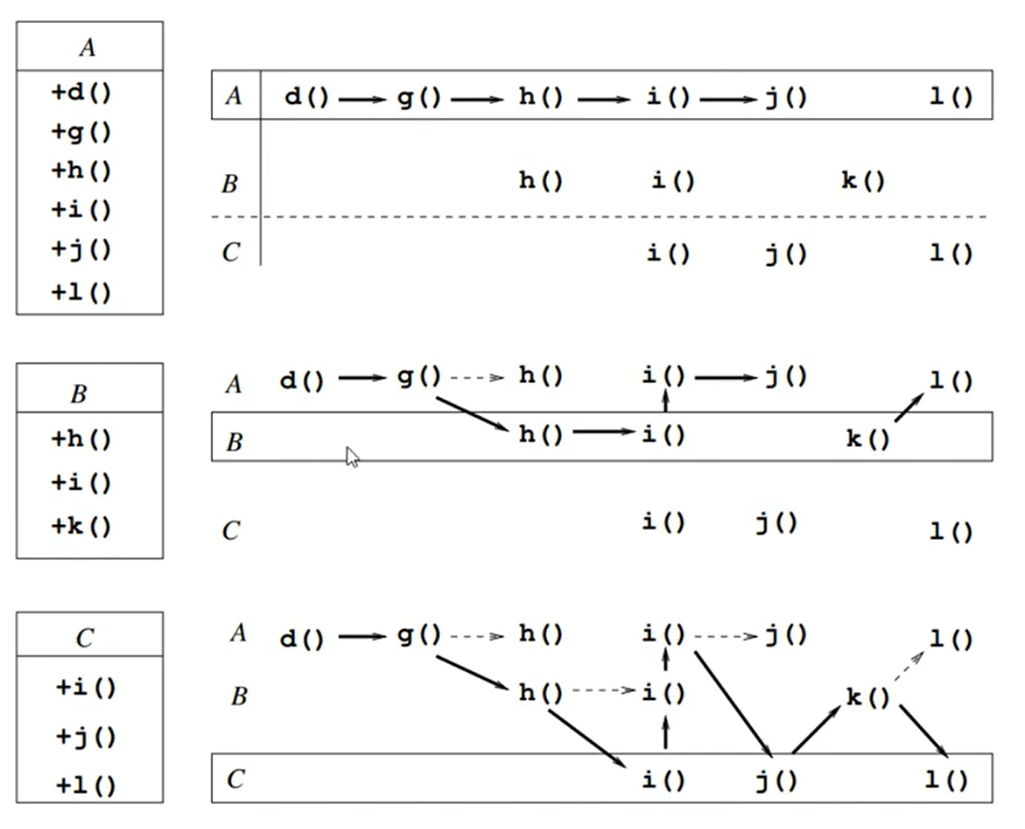
\includegraphics[width=0.7\linewidth]{Degree//static/ST_yo_yo_graph.png}
        \caption{Yo-Yo graph example}
    \end{figure}
\end{itemize}

\subsection{Faults and Anomalies}
\begin{itemize}
    \item Complexity is relocated to the connections among components.
    \item Many faults can now only be detected at runtime.
    \item We are assuming that an anomaly/fault is manifested through polymorphism in a context that uses an instance of an ancestor, i.e., instances of descendant classes can be substituted for instances of the ancestor.
    \item Faults described are language independent.
    \item \textbf{Inconsistent type use fault (ITU)}: A descendant class does not override any inherited method.
    \item \textbf{State Definition Anomaly (SDA)}: The state interactions of a descendant are not consistent with those of its ancestor. The refining methods fail to define some variables and hence required definitions might not be available.
    \item \textbf{State Definition Inconsistency Anomaly (SDIH)}: A local variable is introduced to a class definition and the name of the variable is the same as an inherited variable $v$. A reference to $v$ will refer to the descendant's $v$.
    \item \textbf{State Visibility Anomaly (SVA)}: Consider a class W, which is an ancestor X and Y, X extends W and Y extends W. W declares a private variable v, v is defined by $W::m$. Y overrides $m()$, and calls $W::m()$ to define v. This causes a data flow anomaly as v is private for W.
    \item \textbf{State Defined Incorrectly}: An overriding method defines the same state variable that the overridden method defines. In the absence of identical computations by the two methods, this could result in a behavior anomaly.
    \item \textbf{Indirect Inconsistent State Definition Fault}: A descendant adds an extension method that defines an inherited state variables.
\end{itemize}

\subsection{Coupling Criteria}
\begin{itemize}
    \item \textbf{Coupling variables}: Variables defined in one unit and used in another unit.
    \item \textbf{Coupling Sequences}: Pairs of method calls within body of method under test.
    \begin{enumerate}
        \item Made through a common instance context.
        \item With respect to a set of state variables that are commonly referenced by both methods.
        \item Consists of at least one coupling oath between the two method calls with respect to a particular state variable.
    \end{enumerate}
    \item These coupling sequences represent potential state space interactions between the called methods with respect to calling method.
    \item A reference $o$ can refer to instances whose actual instantiated types are either the base type of $o$ or a descendant of $o$'s type.
    \item $o$ is considered to be defined when one of the state variables $v$ of $o$ is defined.
    \item Definitions and uses in object-oriented applications for coupling variables can be indirect.
    \item Indirect definitions and uses occur when a method defines or references a particular value $v$.
    \item \textbf{Polymorphic call set} or \textbf{Satisfying set}: Set of methods that can potentially execute as result of a method call through a particular instance context.
    \item The calling method is the \textbf{coupling method} $f()$, it calls $m()$, the \textbf{antecedent method}, to define a variable, and $n()$, the \textbf{consequent method}, to use the variable.
    \item \textbf{Transmission set}: Variables for which a path is def-clear.
    \item \textbf{Coupling set} is the intersection of the variables defined by $m()$, used by $n()$.
    \item \textbf{All-Coupling-Sequences (ACS)}: For every coupling sequence $S_j$ in $f()$, there is at least one test case $t$ such that there is a coupling path induced by $S_{j,k}$ that is a sub-path of the execution trace of $f(t)$.
    \item At least one coupling path must be executed. Does not consider inheritance and polymorphism.
    \item \textbf{All-Poly-Classes (APC)}: For every coupling sequence $S_{j,k}$ in method $f()$, and for every class in the family of types defined by the context of $S_{j,k}$, there is at least one test case $t$ such that when $f()$ is executed using $t$, there is a path $p$ in the set of coupling paths of $S_{j,k}$ that is a sub-path of the execution trace of $f(t)$.
    \item At least one test for every type the object can bind to. Include instance contexts of calls.
    \item \textbf{All-Coupling-Defs-and-Uses (ACDU)}: For every coupling variable $v$ in each coupling $S_{j,k}$ of $t$, there is a coupling path induced by $S_{j,k}$ such that $p$ is a sub-path of the execution trace of $f(t)$ for at least one test case $t$.
    \item Every last definition of a coupling variable reaches every first use. Does not consider inheritance and polymorphism.
    \item \textbf{All-Poly-Coupling-Defs-and-Uses (APDU)}: For every coupling sequence $S_{j,k}$ in $f()$, for every class in the family of types defined by the context of $S_{j,k}$, for every coupling variable $v$ of $S_{j,k}$, for every node $m$ that has a last definition of $v$ and every node $n$ that has a first-use of $v$, there is a path $p$ in the coupling paths of $S_{j,k}$, that is a sub-path of the trace of $f()$.
    \item Every last definition of a coupling variable reaches every first use for every type binding. Handles inheritance and polymorphism.
    \begin{figure}[H]
        \centering
        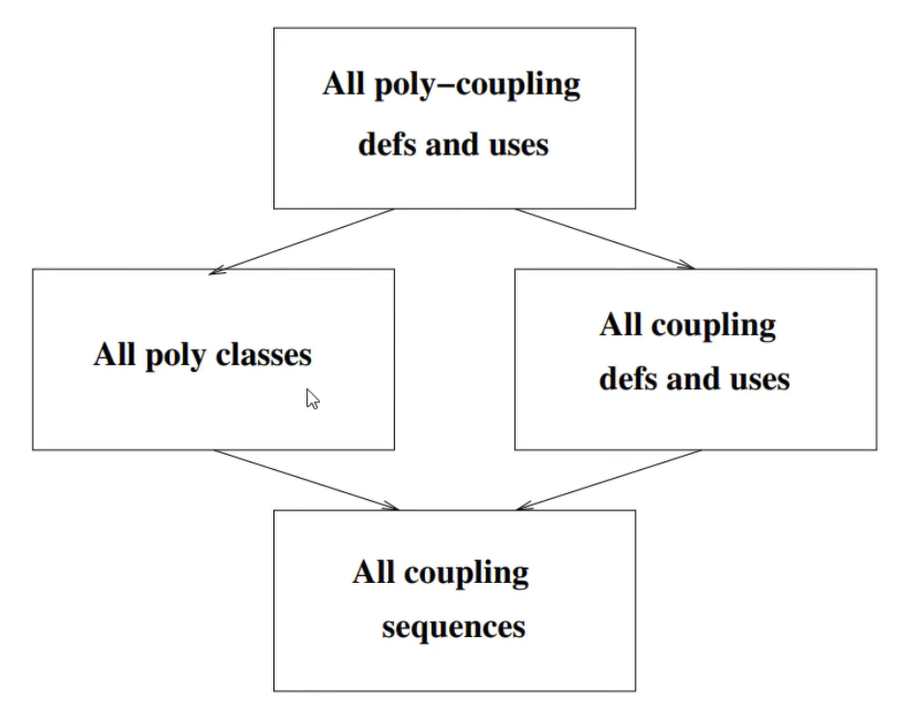
\includegraphics[width=0.5\linewidth]{Degree//static/ST_OO_subsumption.png}
        \caption{Object-Oriented Subsumption}
    \end{figure}
\end{itemize}

\section{Web Application Testing}
\subsection{Introduction}
\begin{itemize}
    \item A \textbf{web application} is a program that is deployed on the web.
    \item It is like a client-server application where the client runs in a web browser.
    \item Composed of independent, loosely coupled software components.
    \item Inherently concurrent and often distributed.
    \item Most components are relatively small.
    \item Uses numerous new technologies, often mixed together.
    \item \textbf{Presentation layer}: HTML, output and UI.
    \item \textbf{Data content layer}: Computation, data access.
    \item \textbf{Data representation layer}: In-memory data storage.
    \item \textbf{Date storage layer}: Permanent data storage.
    \item Web applications are heterogeneous, dynamic and must satisfy very high quality attributes.
    \item Security breaches on web applications are also a major concern.
    \item HTTP is a stateless protocol, each request is independent of previous request.
    \item State is managed by using cookies, session objects, etc.
    \item Servers have little information about where a request comes from.
    \item Users can change the flow of control arbitrarily.
    \item A \textbf{web service} is a system of software that allows machines to interact with each other through a network.
    \item Typically used to achieve reusability of application components. Many web services don't have user interfaces.
    \item A \textbf{web page} contains HTML content that can be viewed in a single browser window.
    \item A \textbf{website} is a collection of web pages and associated software elements that are related semantically by content and syntactically through links and other control mechanism.
    \item A \textbf{static web page} is unvarying and the same to all users.
    \item A \textbf{dynamic web page} is created by a program on demand.
    \item A \textbf{test case for a web application} is a sequence of interactions between components on clients and servers. They are paths of transitions through the web applications.
    \item Testing for static websites
    \begin{enumerate}
        \item This is not program testing, but checking that all the HTML connections are valid.
        \item The main issue to test for is \textbf{dead links}, i.e., links to URLs that are no longer valid.
        \item We should also evaluate several non-functional parameters: Load testing, Performance evaluation, Access control issues.
    \end{enumerate}
    \item Nodes are web pages, and edges are HTML links.
    \item The graph is built by starting with an introductory page and recursively doing BFS of all links from that page. This graph is tested for edge coverage.
\end{itemize}

\subsection{Client-Side Testing}
\begin{itemize}
    \item The user interface is on the client and the actual software is on the server.
    \item Tester typically has no access to data, state or the source code on the server.
    \item Test inputs are HTML form elements.
    \item Inputs can be generated or chosen.
    \item \textbf{Bypass testing}: Values that violate constraints on the inputs, as defined by client-side information.
    \item Bypass testing creates inputs that intentionally violate these validation rules and constraints.
    \item The basic idea in \textbf{bypass testing} is to let a tester save and modify the HTML.
    \item Server side inputs can be modified too, but, can be risky if they corrupt data in the server.
    \item Client side input validation is performed by HTML form controls, their attributes and client side scripts that access DOM.
    \item Validation types are categorized as HTML and scripting.
    \item HTML supports syntactic validation.
    \item Client scripting can perform both syntactic and semantic validation.
    \item \textbf{Value level bypass testing} tries to verify if a web application adequately evaluates invalid inputs.
    \item \textbf{Parameter level bypass testing} tries to check for issues related to relationships among different parameters of an input.
    \item \textbf{Control flow level bypass testing} tries to verify web applications by executing test cases that break the normal execution sequence.
    \item A testing approach that uses data captured during \textbf{user sessions} to create test cases.
    \item User-session data based testing reduces the effort involved when test engineers are required to generate test cases.
    \item Let $U=\{u_1,u_2,...,u_m\}$ be a set of user sessions, with $u_i$ consisting of $n$ requests $r_1,r_2,...,r_n$, where each $r_i$ consists of $url[name-value]^*$
    \item We define a user session as beginning when a request from a new IP address reaches the server and ending when the user leaves the website or the session times out.
    \item Collect all client request information. This can be accomplished based on the underlying web application development technologies used.
    \item Three stand-alone variants of the basic approach involving direct use of the session data.
    \begin{enumerate}
        \item Directly reuse entire sessions: Transform each $u_i\in U$ into a test case by formatting each of its associated requests $r_1,r_2,...,r_n$ into an HTTP request that can be sent to a web server. The resulting test suite contains $m$ test cases, one for each user session.
        \item Replay a mixture of sessions: Select an unused session $u_a$ from $U$.\\
        Copy requests $r_1$ through $r_i$ from $u_a$, where $i$ is a random number, into the test case.\\
        Randomly select session $u_b$ from $U$, where $b\neq a$, and search for any $r_j$ in $u_b$ with same URL as $r_i$.\\
        If not $r_j$ found then consider direct reuse, else add all the requests following $r_j$ from $u_b$ into the test case after $r_i$.\\
        Mark $u_b$ as used and repeat the process until no more unused sessions are available in $U$.
        \item Replay sessions with some targeted modifications: Replay user sessions by modifying the input forms that can alter the behavior of the web application.\\
        Select an unused session $u_a$ from $U$.\\
        Randomly select an unused request $r_i$ from $u_a$. If there are no more unused $r_i$ in $u_a$, then reuse $u_a$ directly as a test case.\\
        If $r_i$ does not contain at least one name-value pair, mark $r_i$ as used and repeat previous step.\\
        If $r_i$ has one or more name-value pairs, then modify the name-value pairs, create test cases.\\
        Mark $u_a$ as used and repeat process until no more.
    \end{enumerate}
    \item Two hybrid variants that combine the basic approach with other functional testing techniques.
\end{itemize}

\subsection{Server-Side Testing}
\begin{itemize}
    \item \textbf{Valid responses}: Invalid inputs are adequately processed by the server.
    \item \textbf{Faults and failures}: Invalid inputs cause abnormal server error.
    \item \textbf{Exposure}: Invalid inputs are not recognized by the server and abnormal software behavior is exposed to users.
    \item If server-side source code is available, we can use graph models to test the server.
    \item CFG exhibit only static models, not effective for web applications.
    \item \textbf{Presentation layer} of a web application contains software that is useful to do testing.
    \item \textbf{Component Interaction Model (CIM)}: Models individual components, combines atomic sections, intra-component.
    \item An \textbf{atomic section} is a section of HTML with the property that if any part of the section is sent to a client, the entire section is. A HTML file is an atomic section.
    \item A \textbf{content variable} is a program variable that provides data to an atomic section.
    \item \textbf{Application Transition Graph (ATG)}:Each node is one CIM, Edges are transitions among CIMs, Inter-component.
    \item Atomic sections are combined to model dynamically generated web pages.
    \item $\Gamma$: Finite set of web components
    \item $\Theta$: Set of transitions among web software components
    \item $\Sigma$: Set of variables that define the web application state
    \item $\alpha$: Set of start pages
    \item \textbf{Simple Link Transition}: An HTML link
    \item \textbf{Form Link Transition}: Form submission link
    \item \textbf{Component Expression Transition}: Execution of a software component causes a component expression to be sent to the client.
    \item \textbf{Operational Transition}: A transition out of the software's control.
    \item \textbf{Redirect Transition}: Server side transition, invisible to user.
\end{itemize}
\pagebreak

\section{Miscellaneous Testing}
\subsection{Regression Testing}
\begin{itemize}
    \item \textbf{Regression testing} is the process of validating modified software to detect whether new errors have been introduced into previously tested code and to provide confidence that modifications are correct.
    \item Black-box testing, typically very expensive and well-used.
    \item Let $P$ be a procedure or program. Let $P'$ be a modified version of $P$ and let $T$ be a test suite for $P$
    \item Select $T'\subseteq T$, a set of test cases to execute on $P'$.
    \item This involves the \textbf{regression test selection} problem.
    \item Test case $t$ is \textbf{obsolete} for program $P'$ iff $t$ specifies an input to $P$ that is invalid for $P'$, or $t$ specifies an invalid input-output relation for $P'$. Identify these and remove from $T$.
    \item Test $P'$ with $T'$, establishing $P'$s correctness with respect to $T'$
    \item If necessary create $T"$, a set of new functional or structural test cases for $P'$
    \item This involves \textbf{coverage identification} problem.
    \item Test $P'$ with $T"$, establishing $P'$s correctness with respect to $T"$.
    \item Create $T"'$, a new test suite and test execution profile for $P'$, from $T,T'$, and $T"$.
    \item This involves the \textbf{test suite maintenance} problem.
    \item And we also have the \textbf{test suite execution} problem.
    \item \textbf{Minimization test selection techniques} for regression testing attempt to select minimal sets of test cases from $T$ that yield coverage of modified or affected portions of $P$.
    \item \textbf{Data-flow coverage based regression test selection} techniques select test cases that exercise data interactions that have been affected by modifications.
    \item Techniques that are not safe can fail to select a test that would have revealed a fault in the modified program.
    \item \textbf{Random Techniques}: Randomly select test cases, often useless.
    \item The \textbf{retest-all} technique simply reuses all existing test cases.
    \item Cerberus Testing is a good open source tool.
\end{itemize}

\subsection{Software Quality Metrics}
\begin{itemize}
    \item \textbf{Software quality} is the capability of a software product to conform to its requirements.
    \item \textbf{Software function quality}: Reflects how well it complies with or conforms to a given design, based on functional requirements or specifications.
    \item \textbf{Software structural quality}: Refers to how it meets non-functional requirements that support the delivery of the functional requirements, such as robustness or maintainability.
    \item \textbf{Software Quality Assurance}: A set of activities to ensure the quality in software engineering processes that ultimately result in quality software products.
    \item \textbf{Software Quality Control}: A set of activities to ensure the quality of software products.
    \item A \textbf{software metric} is a measure of the degree/extent to which a software system or process possesses some property.
    \item \textbf{Product metrics}: Describe the various characteristics of the software, size, complexity, metric related to design.
    \item \textbf{Process metrics}: Describe all the characteristics that can be used to improve the development of software and its maintenance.
    \item \textbf{Project metrics}: Describe the characteristics of the project and its execution, team size, cost, schedule, productivity.
    \item Number of lines of code(KLOC), Cyclomatic complexity, Program size.
    \item \textbf{Coupling}: Coupling is the degree of interdependence between software modules, it is a measure of how closely connected two modules are.
    \item \textbf{Cohesion}: Cohesion is a measure of the strength of relationship between the methods and data of a class.
    \item \textbf{Mean time to failure}: The time between failures. Used mainly in safety critical systems.
    \item \textbf{Defect Density}: Measures the number of defects relative to the size of software (KLOC/function points)
    \item \textbf{Issues reported by/related to customers}: Number of issues per unit of time, as reported by customers.
    \item \textbf{Satisfaction of customers}: Measured through a survey on a five-point scale.
    \item \textbf{Defect Removal Effectiveness} is defined as
    \begin{equation*}
        DRE=\frac{\text{Defects removed during a development phase}}{\text{Defects latent in the product}}\times 100\%
    \end{equation*}
    \item Fix backlog and backlog management using Backlog Management Index
    \begin{equation*}
        BMI=\frac{\text{Number of problems closed during the month}}{\text{Number of problems arrived during the month}}\times 100\%
    \end{equation*}
\end{itemize}

\subsection{Non-Functional Testing}
\begin{itemize}
    \item \textbf{Interoperability testing} determines whether the system can interoperate with other third-party products. Can involve \textbf{compatibility testing} too.
    \item Forward and Backward compatibility.
    \item \textbf{Security testing} determines if a system products data and maintains security related functionality as intended.
    \item \textbf{Confidentiality}: Requirement that data and processes by protected from unauthorized disclosure.
    \item \textbf{Integrity}: Requirement that data and processes be protected from unauthorized modification.
    \item \textbf{Availability}: Requirement that data and processes be protected from denial of service to authorized users.
    \item Also deals with \textbf{authorization} and \textbf{authentication} verification.
    \item Verify that only authorized accesses to the system are permitted.
    \item Verify the correctness of encryption and decryption algorithms for systems where data/messages are encoded.
    \item Verify that illegal reading of files, to which the perpetrator is not authorized is not allowed.
    \item Ensure that virus checkers prevent/curtail entry of viruses into the system.
    \item Identify back doors in the system left open by developers. Test for access through back doors.
    \item Verify different authentication, client server communication, wireless security protocols etc.
    \item \textbf{Reliability tests} measure the ability of system to keep operating over specified periods of time.
    \item \textbf{Scalability testing} verifies that a system can scale up to its engineering limits.
    \item \textbf{Documentation testing} is done to verify the technical accuracy and readability of various documentation including user manuals, tutorials, online help etc.
    \item \textbf{Read test}: A documentation is reviewed for clarity, organization, flow and accuracy without executing the documented instructions on the system.
    \item \textbf{Hands-on test}: Online help is exercised, error messages verified to evaluate their accuracy and usefulness.
    \item \textbf{Functional test}: Instructions embodied in the documentation are followed to verify that the system works as it has been documented.
    \item  Each country has regulatory bodies guiding the availability of a product in that country.
    \item \textbf{Performance testing} is done to determine the system parameters in terms of responsiveness and stability under various workloads.
    \item \textbf{Soak testing} is endurance testing and \textbf{spike testing} is stress testing.
    \item \textbf{Test Driven Development}: Write tests cases then code for those test cases. As code size increases, do \textbf{re-factoring}.
\end{itemize}

\end{document}